%                                                                 aa.dem
% AA vers. 9.1, LaTeX class for Astronomy & Astrophysics
% demonstration file
%                                                       (c) EDP Sciences
%-----------------------------------------------------------------------
%
%\documentclass[referee]{aa} % for a referee version
%\documentclass[onecolumn]{aa} % for a paper on 1 column  
%\documentclass[longauth]{aa} % for the long lists of affiliations 
%\documentclass[letter]{aa} % for the letters 
%\documentclass[bibyear]{aa} % if the references are not structured 
%                              according to the author-year natbib style

%
\documentclass{aa}  

%
\usepackage{graphicx}
%%%%%%%%%%%%%%%%%%%%%%%%%%%%%%%%%%%%%%%%
\usepackage{txfonts}
%%%%%%%%%%%%%%%%%%%%%%%%%%%%%%%%%%%%%%%%
\usepackage[hyperindex=true,breaklinks=true,colorlinks=true,linkcolor=blue,filecolor=blue,urlcolor=blue,citecolor=blue,breaklinks=true]{hyperref}
% To add links in your PDF file, use the package "hyperref"
% with options according to your LaTeX or PDFLaTeX drivers.
%

\usepackage{tabularray}
\usepackage{placeins}
\usepackage{float}


\begin{document} 


   \title{Deriving Star Formation Histories of Galaxies from  Spectra with Simulation-based Inference}

   \titlerunning{Star Formation Histories from  Spectra with Simulation-based Inference}

   \subtitle{}

   \author{Patricia Iglesias-Navarro \inst{1,2}   \and Marc Huertas-Company \inst{1,2,3,4} \and Ignacio Martín-Navarro \inst{1,2} \and Johan H. Knapen \inst{1,2} \and Emilie Pernet \inst{1,2,5}}

   %check order and more authors

   \institute{Instituto de Astrofísica de Canarias, C/ Vía Láctea s/n, 38205 La Laguna, Tenerife, Spain \and Departamento de Astrofísica, Universidad de La Laguna, 38200 La Laguna, Tenerife, Spain \and
             Observatoire de Paris, LERMA, PSL University, 61 avenue de l'Observatoire, F-75014 Paris, France
          \and  
          Universit\'e Paris-Cit\'e, 5 Rue Thomas Mann, 75014 Paris, France \and
    Department of Physics, Faculty of Engineering and Physical Sciences, University of Surrey, GU2 7XH, Guildford, United Kingdom}


   \date{}

% \abstract{}{}{}{}{} 
% 5 {} token are mandatory
 
  \abstract
   {High-resolution galaxy spectra encode information about the stellar populations within galaxies. The properties of the stars, such as their ages, masses,  and metallicities, provide  insights into the underlying physical processes that drive the growth and transformation of galaxies over cosmic time.
    We explore an amortised implicit inference approach to estimate from optical absorption spectra the posterior distributions of metallicities and star formation histories (SFHs) of galaxies, i.e. star formation rate as a function of time. 
    We generate a sample of synthetic spectra to train and test our model in a simulation-based inference workflow using the spectroscopic predictions of the MILES stellar population library and non-parametric SFHs. We reliably estimate the mass assembly of an integrated stellar population with well-calibrated uncertainties. Specifically, we reach a score of accuracy of $0.97\,R^2$ for the time at which a given galaxy from the test set formed $50\%$ of its stellar mass, obtaining samples of the posteriors in only $10^{-4}$\,s. We then apply the pipeline to real observations of  massive elliptical galaxies, recovering the well-known relationship between the age and the velocity dispersion, and show that the most massive galaxies ($\sigma\sim300$ km/s) build up to 90\% of their total stellar masses $1$\,Gyr after the Big Bang. The measurements also agree with the state-of-the-art inversion codes, but the inference is performed up to five orders of magnitude faster.
    This machine learning-based implicit inference applied to full spectral fitting makes it possible to address large number of galaxies while performing a thick sampling of the posteriors. It allows to estimate both the deterministic trends and the inherent uncertainties of the highly degenerated inversion problem, so far inaccessible, dealing with the size and complexity of upcoming spectroscopic surveys such as DESI, WEAVE or 4MOST.}
    
   \keywords{galaxies: evolution - galaxies: statistics}

   \maketitle
%
%-------------------------------------------------------------------

\section{Introduction}

 Understanding the physical processes that regulate star formation over cosmic time is one of the main challenges of galaxy studies, as their evolution depends on a balance between processes that trigger star formation and others that prevent it by expelling or heating gas \citep[e.g.][]{Franx90,Silk_2012, lilly13, nacho}. Reconstructing SFHs is thus a fundamental step towards understanding galaxy evolution. However, inferring  from observed spectra for a statistically significant sample of galaxies is a complex inverse problem subject to a large number of degeneracies which are not well understood \citep[e.g.][]{worthey92, Ocvirk, Conroy_2009}. \\

  Stellar population synthesis (SPS) models are normally used, the building blocks of which are simple stellar populations (SSPs). SSPs describe the evolution in time of the spectrum of a single stellar burst of fixed metallicity and chemical abundance, requiring three basic inputs: stellar evolution theory in the form of isochrones, e.g., Padova \citep{Girardi_2000}, BaSTI \citep{Pietrinferni_2006}, or MIST \citep{Choi_2016};  empirical or  theoretical stellar spectral libraries, e.g., CaT \citep{Cenarro_2001}, MILES \citep{Vazdekis_2010}, or XSL \citep{Gonneau_2020}; and an IMF \citep{salpeter95,Kroupa_2001,Chabrier_2003}, each of which may in principle depend on metallicity and/or elemental abundance patterns.  Composite stellar populations (CSPs) differ from simple ones because they contain stars with a range of ages given by their SFHs and with a range of metallicities as given by their time-dependent metallicity distribution function $P$($\rm{[M/H]}$\footnote{i.e. metals over hydrogen, defined as $\rm{[M/H]}=\log \left(\frac{\rm M}{\rm H}\right)-\log \left(\frac{\rm M}{\rm H}\right)_{\odot}$.}, $t$).\\



To connect a model with observations, a statistical inference framework is required. Full spectral fitting algorithms are a popular tool to infer stellar population properties from integrated spectra, generally based on a backward comparison between data and models  \citep[e.g.][]{starlight,Ocvirk,vespa,firefly, Cappellari2022}. The success and reliability of this method depends on the quality of the template spectra, and of the robustness of the fitting algorithm. In parallel, stellar population inversion algorithms have evolved into Bayesian statistics \citep[e.g.][]{Mart_n_Navarro_2019,Johnson_2021,2024maciata, 2024wang}, using primarily the Markov Chain Monte Carlo (MCMC) method for sampling the posterior distributions, which are assumed to be Gaussian, allowing an efficient exploration of the degeneracies associated with the large parameter space.\\ 

Existing Bayesian spectral modelling approaches, however, require a substantial computational investment, ranging from $10$ - $100$ CPU hours per galaxy \citep{Carnall_2019,tacchela21}. Although this computational demand is already high for current datasets, like SDSS \citep{SDSS} or COSMOS \citep{cosmos}, containing hundreds of thousands of galaxy spectral energy distributions (SEDs), it becomes a prohibitive bottleneck for upcoming surveys. Over the next decade, DESI \citep{desi}, WEAVE \citep{weave}, 4MOST \citep{4most}, and MOONS \citep{MOONS} will capture spectra from billions of galaxies, which would imply tens or hundreds of billions of CPU hours.\\

Machine learning-based models are becoming more popular in astronomy \citep[e.g.][]{huertascompany2023brief, joanna24,moser24,hunt2024predicting}. In contrast with traditional spectral fitting, where SFHs are built from some ensemble of SSPs to recreate the spectra, machine learning directly learns the relationship between the observed features and the entire SFHs. Its systematic uncertainties are thus independent of those from spectral fitting, complementing and strengthening the measurements \citep{lovell19}. On the other hand, neural density estimators have recently been introduced to address the computational challenge of Bayesian methods \citep[e.g.][]{kwon24}, demonstrating a significant acceleration in SED model evaluations of up to five orders of magnitude \citep{Hahn_2022}, so the posterior inference for each galaxy now takes seconds.\\


In this work, we explore a novel approach based on probabilistic machine learning and likelihood-free inference to estimate the SFHs of galaxies from their optical absorption spectra.  The main advantage over classical Bayesian inference methods is that our approach does not assume a functional form for likelihood, typically considered Gaussian, and that once the model is trained, it can be evaluated on different observations with minimal computational cost. The outline of the paper is as follows: in Sect.~\ref{methods} we describe the Bayesian inference framework, using SPS (\ref{forward}), an encoder of the spectra (\ref{encoder}),  and a neural density estimator (\ref{normflows}). In Sect.~\ref{results} we test the model in both mocked observations and stacks of early-type galaxies from SDSS. We further discuss the details of the model and the measurements of the stacks' physical properties in Sect.~\ref{discussion}.


%--------------------------------------------------------------------
\section{Methods}
\label{methods}

When applied to spectral fitting, Bayesian algorithms aim to infer the posterior probability distributions $P(\theta \mid x)$ of galaxy properties, $\theta$, given observations, $x$. For a specific $\theta$ and $x$, one typically evaluates the posterior using Bayes' rule, $P(\theta \mid x) \propto P(\theta) \; P(x \mid \theta)$, where $P(\theta)$ denotes the prior distribution and $P(x \mid \theta)$ the likelihood, usually assumed to have a Gaussian functional form:


\begin{equation}
\log P(x \mid \theta)=-\frac{1}{2}(x-m(\theta))^T C^{-1}(x-m(\theta)),
\end{equation}




where $m(\theta)$ is the theoretical model, in our case a galaxy spectral model, and $C$ is the covariance matrix of the observations. \\

Simulation-based inference (SBI), also known as likelihood-free inference, offers an alternative that requires no assumptions about the form of the likelihood. In a nutshell, it consists of creating synthetic data, often called the forward model,  and then fitting them like real observations, the backward model, comparing against a known ‘truth’. Therefore, SBI uses a generative model, i.e. a simulation $F$, to generate mock data $x^{\prime}$ given parameters $\theta^{\prime}: F\left(\theta^{\prime}\right)=x^{\prime}$. It uses a large number of simulated pairs $\left(\theta^{\prime}, x^{\prime}\right)$ to directly estimate either the posterior $P(\theta \mid x)$, the likelihood $P(x \mid \theta)$, or the joint distribution of the parameters and data $P(\theta, x)$. This technique has already been applied successfully to several Bayesian parameter inference problems in astronomy \citep[e.g.][]{Cameron_2012, mishrasharma2022inferring, hahn23,zhang23}.\\

 The SBI approach can help us deal with the parameter space coverage, as most observations are unbalanced and affected by selection effects, and do not allow to obtain the kind of broad and uniform dataset usually required by inference algorithms. Moreover, SBI is especially useful when testing single-effect biases (e.g., parametrizations of SFHs or noise), enabling to layer complexity. In contrast, it is likely to generate problems of domain shifts when generalising results to real observations. Modelling considerations, like priors, wavelength coverage, or resolution, can have a significant impact on inferred galaxy properties \citep{Leja_2019,Hahn_2022} and must be carefully selected.\\ 


\subsection{Forward model}
\label{forward}

The first step is to generate a synthetic dataset to train and test our model, for which the spectrum, the SFH, and the metallicity are known. We work with MILES SPS models \citep{Vazdekis_2010}.  These fully empirical SSP models provide medium resolution \citep[$\text{FWHM}=2.51\AA$,][]{falcon11} predictions for a wide range of ages (from $0.03$ Gyr to $14.00$ Gyr) and metallicities ($\rm{[M/H]}$ moving from $-2.27$ to $0.40$). We select a Kroupa universal IMF and BaSTI isochrones, in the wavelength range $[3540.5,7409.6] \, \AA$, and use the so-called base models for $[\alpha/\rm{Fe}]$, following the abundance pattern of the solar neighbourhood.\\

We build physically-motivated non-parametric SFHs with Dense Basis \citep{Iyer_2017}, specifically the module GP-SFH. These SFHs allow complex behaviours like rejuvenation events, bursts or sudden quenching, and do not rely on a fixed functional form. The selected prior assumes that the fractional specific SFR (sSFR, i.e. the SFR normalised by the stellar mass), for three equally spaced time bins, follows a Dirichlet distribution \citep{Leja_2017} with a concentration parameter $\alpha=1$. Moreover, a uniform prior is included for the logarithm of the total stellar mass, $8.0 \leq \text{log} \left(M_{*}/M_{\odot}\right) \leq 12.0$, and for the logarithm of the sSFR at $z=0$, $-17.0 \leq \text{log} \left(\text{sSFR}/ \rm{yr}^{-1}\right) \leq -7.5$. We believe that these priors are general enough not to impose strong effects on the measurements, however, they will always play a role in the model predictions.\\


For simplicity we assume that there is no time evolution in metallicity, so each SFH is assigned with a single value of $\rm{[M/H]}$. We interpolate MILES spectra in time to obtain a SSP spectrum each $0.01347$ Gyr, with cosmic time in the range $[0.00,13.47]$ Gyr ($1{,}000$ time bins). In addition, as the metallicity bins of the spectral library are not equally spaced, which may cause problems when introducing the spectra to the network, we interpolate them in $\rm{[M/H]}$ too, obtaining $15$ equally spaced values of this parameter in the range $[-2.3,0.4]$. For each artificial SFH, given a value of $\rm{[M/H]}$, all the MILES interpolated spectra (corresponding to different ages and with that metallicity) are combined as:

\begin{equation}
\resizebox{.49 \textwidth}{!} 
{$
F_{\text{gal}} \left( \lambda,M_{\text{tot}},\rm{[M/H]},[\alpha / Fe]_{\text{Base}} \right) =\displaystyle \sum_{t_i} \frac{M(t_i)}{M_{\text{tot}}} \cdot F_{\text{SSP}} \left( \lambda,t_i,{\rm{[M/H]}},[\alpha/\rm{Fe}]_{\text{Base}}  \right)
$.}
\end{equation}

Finally, each spectrum is normalised by its median. In total, we obtain $10{,}000$ SFHs for each value of $\rm{[M/H]}$, so: $10{,}000$ SFHs x $15$ bins of metallicity $= 150{,}000$ spectra, for which SFHs and metallicities are known. Examples of the mock SFHs and their corresponding spectra are shown in Fig.~\ref{input}.\\

\begin{figure*}[h]
    \centering
    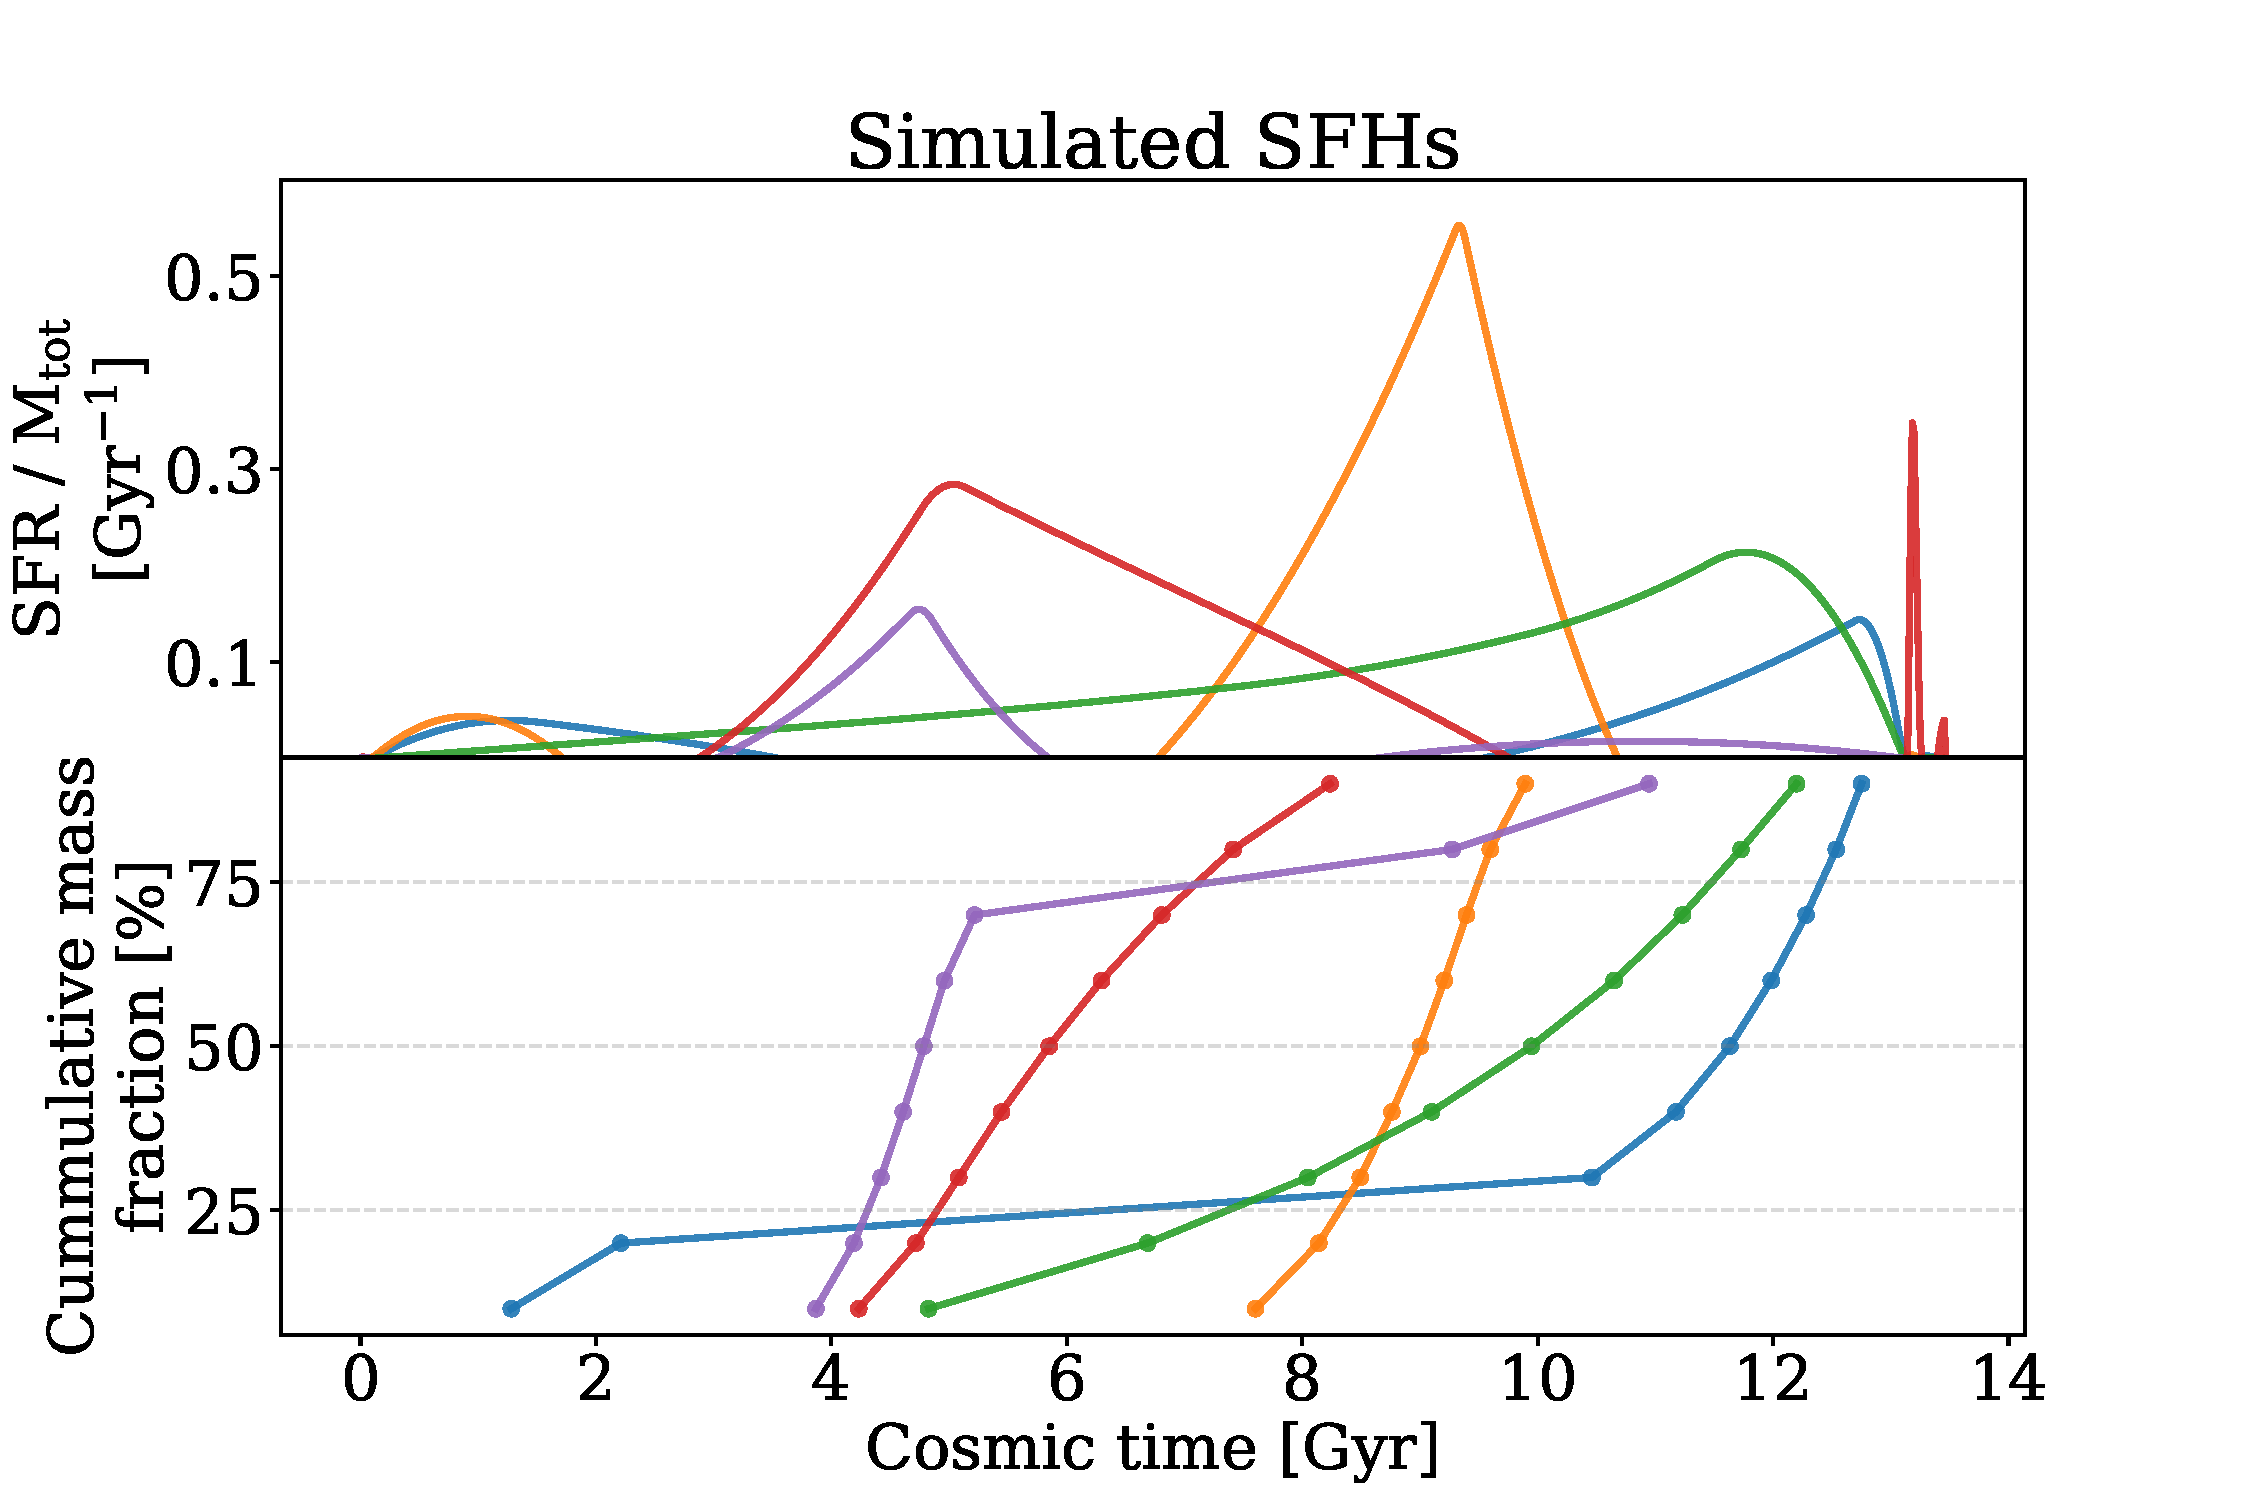
\includegraphics[width=0.49\textwidth]{images/input/sim_sfhs.pdf}
    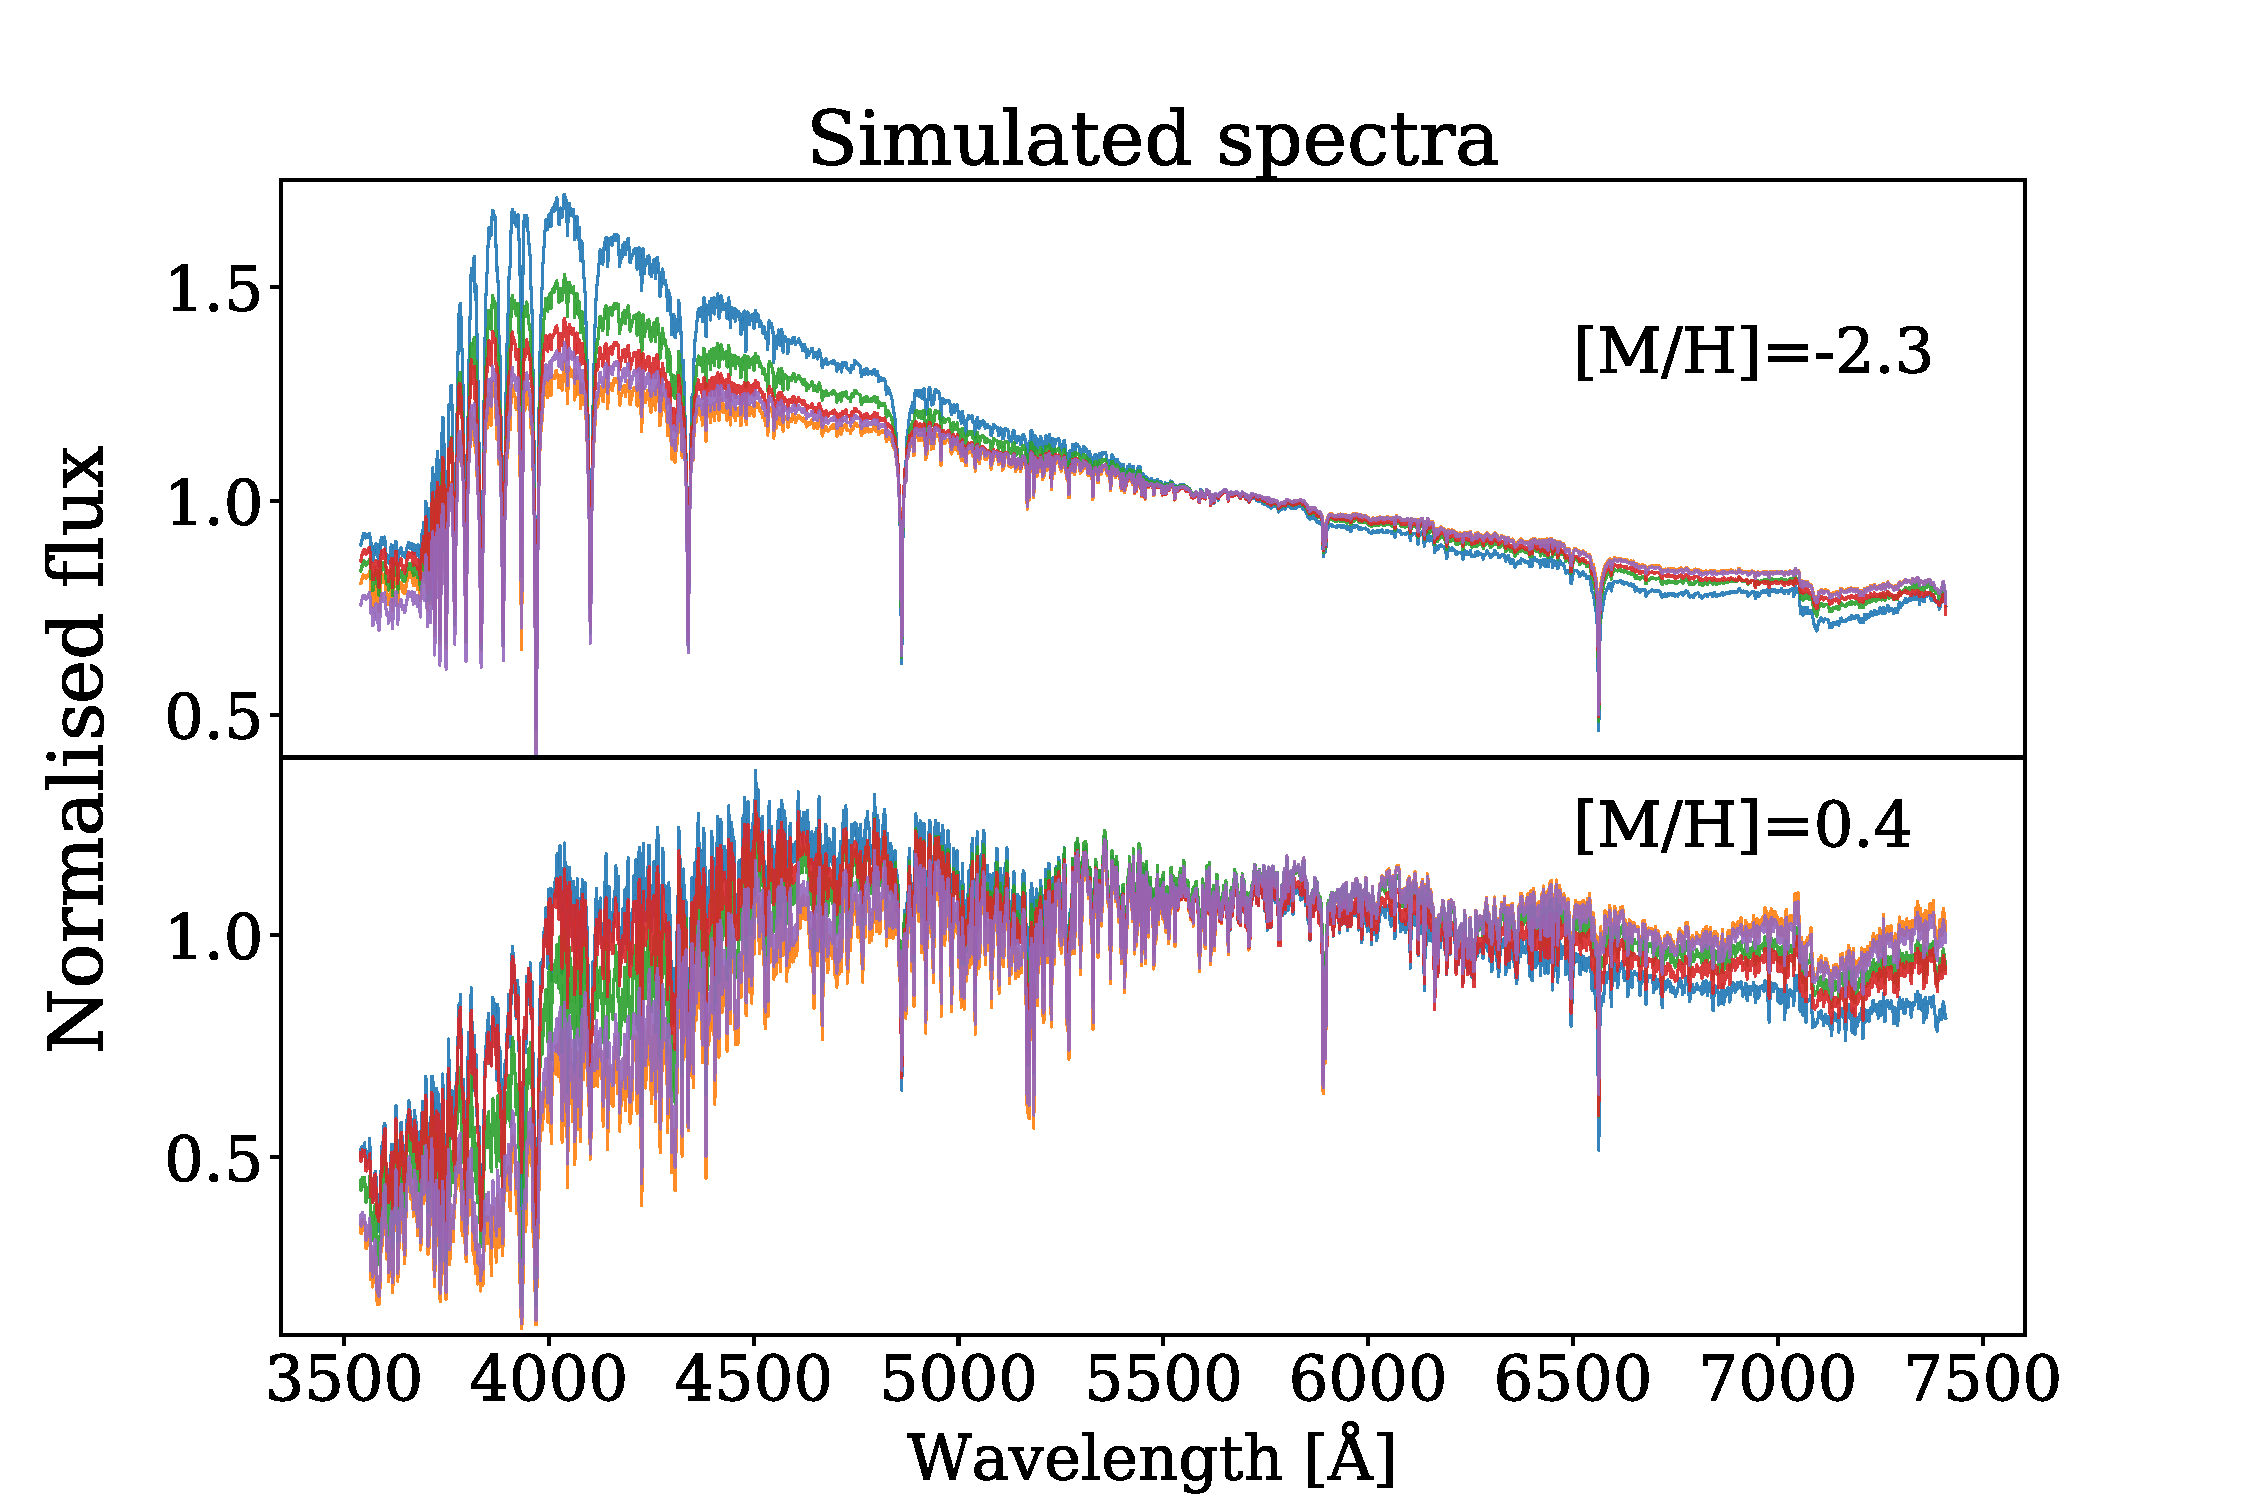
\includegraphics[width=0.49\textwidth]{images/input/sim_spectra.pdf}
    \caption{Samples of the simulated dataset, each of them with a different colour. In the left plot we show their mocked SFHs: in the upper panel the SFR normalised by the total stellar mass in Gyr$^{-1}$, and in the lower one the nine stellar mass percentiles, together with three dashed grey lines indicating when $25\%$, $50\%$ and $75\%$ of the total stellar mass has been formed. In the right plot, we show the  simulated normalised spectra corresponding to these SFHs using the same colours, for two different values of metallicity: in the upper panel we fix $\rm{[M/H]}=-2.3$, and in the lower one  $\rm{[M/H]}=0.4$, which are respectively the minimum and maximum bins of $\rm{[M/H]}$ in the simulation.}
    \label{input}
\end{figure*}


 Stellar mass curves, i.e. SFR as a function of time, are integrated to get nine stellar mass percentiles. We thus focus on the cosmic time,  i.e. the time since the Big Bang, at which $10$\%, $20$\%, ... $90$\%  of the total stellar mass of the galaxy has been formed. These quantities are more robust and smoother than their non-cumulative analogues, possibly relieving the effects imposed by the intrinsic priors of the simulation, so that the model inference is more stable. \\


\subsection{Backward Model}
\label{backward}
\subsubsection{Encoding the spectra}
\label{encoder}

High-quality absorption spectra typically cover, at least, a thousand $\AA$, described by a similar number of pixels. However, the widespread adoption of template libraries suggests that galaxy spectra in fact occupy a low-dimensional manifold. In particular, \cite{Portillo_2020} demonstrated that a high-fidelity reconstruction can be achieved by an autoencoder (AE) architecture  \citep{hinton}, a non-linear dimensionality reduction technique, with a latent space of just six dimensions. \cite{Teimoorinia_2022}  and  \cite{melchior2022} improved the method by introducing convolutional elements into the AE to aid the extraction of correlated features from the spectra. In short, AEs are feed-forward neural networks that learn efficient encodings of data in an unsupervised manner. They consist of two parts: an encoder, which takes data as input and compresses it to produce a low-dimensional latent representation, and a decoder, which takes the latent representations and decompresses them to reconstruct the original data. Due to their non-linear behaviour, AEs can capture non-linear features, such as line widths, with fewer parameters than principal component analysis (PCA) \citep{Yip_2004}, one of the most commonly used techniques. Moreover, unlike line-ratio diagnosis, AEs use the continuum information in the spectra, resulting in an interpretable latent space that shows clear separations between different classes of galaxies, even though they were never given these classifications in training.\\


We take advantage of this approach to obtain low-dimensional representations of the spectra, using the encoder part of the architecture implemented by \cite{melchior2022} (SPENDER). These representations are more suitable than the full spectrum to be introduced into a Bayesian inference model for a fully probabilistic treatment, and to perform meaningful summary statistics. The size of the latent representations is a tunable parameter and depends on what information in the spectrum is relevant to determine the SFHs and metallicity, as well as on the dimension of the spectrum and the performance required. During this work, it is set to $16$, as most of the details of the spectra that contain information relevant to the early star formation of galaxies are extremely subtle.\\

 Our network consists of a three-layer convolutional neural network (moving to wider kernels and including max-pooling), plus an attention module (dot-product), and a three-layer multi-layer perceptron (MLP), to obtain the latent vectors. Furthermore, an additional two-layer MLP is included to optimise the encoding for our final task: to obtain stellar mass percentiles and a value of $\rm{[M/H]}$, incorporating a log-cosh loss function. This computes the difference between the predicted and actual values, driving the evolution of the training. The encoder is trained with the training and validation sets ($80\%$ and $10\%$ of the total number of samples), and the training is stopped when the validation loss reaches a plateau, after 250 epochs approximately. Then, the model is applied to test data (the remaining $10\%$ of the total number of samples, never seen before by the network), producing not only the latent vectors we will use for the Bayesian inference, but also an initial prediction for the mass percentiles and metallicity that we can easily compare with the true ones. These predictions will not be used once we have trained the encoder: they only drive the training process, while the proper measurements of the galaxy properties will be done by the neural density estimator, as detailed below.\\





\subsubsection{Posterior estimation}
\label{normflows}


We use an Amortised Neural Posterior Estimation (ANPE) technique known as Normalising Flows, to estimate the posterior probability distribution for each of the stellar mass percentiles, and for the metallicity. In a few words, variables $(z)$ described by a simple base distribution $P(z)$, such as a multivariate Gaussian, are transformed through a parameterised invertible transformation $x=f(z)$, that has a tractable Jacobian. The target density $P_f(x)$ is then given by the change-of-variables formula as a product of the base density and the determinant of the transformation's Jacobian:

\begin{equation}
P_f(x)=P(z)\left|\operatorname{det} J_{f^{-1}(x)}\right|.
\end{equation}

Several such steps can be stacked, with the probability density `flowing' through the successive variable transformations. The parameters of the transformations during the training of the model are estimated by maximising the log likelihood of the transformed data under the Gaussian distribution $P(z)$, which is indeed tractable:

\begin{equation}
\log P_f(x)=\log P(f^{-1}(x))+\log \left|\operatorname{det} J_{f^{-1}(x)}\right|.
\end{equation}

Otherwise, it would not be possible to compute the loss since $P(x)$ is unknown. Following this pipeline, Normalising Flows have been generalised to model a conditional density such as  the posterior $P(\theta \mid x)$. Following the choice of \cite{Hahn_2022}, we develop a Masked Autoregressive Flow (MAF) \citep{papamakarios2018masked}, implemented with the module SBI \citep{tejerocantero2020sbi},  with five Masked Autoencoder for Distribution Estimation (MADE) blocks, each of them with two hidden layers of $128$ hidden units. In total, the model has a set of $50{,}560$ free parameters $\phi$. Our goal is to determine $\phi$ for the MAF model, so that given galaxy properties $\theta$ and observations $x$, $P_{\phi}\left(\theta \mid x \right)$ accurately estimates the posterior probability distribution $P\left(\theta \mid x \right)$.  In practice, we divide the training data into training and validation sets with a $90/10$ split. We use the Adam optimiser with a learning rate of $5\cdot 10^{-4}$. To prevent overfitting, we evaluate the likelihood of the data points under the base distribution, using the validation data at every training epoch, and stopping the training when that validation likelihood fails to increase after $20$ epochs.\\

 By using this workflow, we train our model with mock synthetic data, and then apply it to observations to obtain promptly posteriors for the SFHs and metallicity, thanks to its amortised\footnote{Not focused on any particular observation. Once we have a trained model, new data can be evaluated without repeating the training, the computationally expensive step.} nature.\\
 
 We are making two important assumptions. First, the simulator $F$ must be capable of generating mock data $x'$ that is practically indistinguishable from the observations $x$, which is the same requirement of any probabilistic modelling approach, but in contrast with likelihood-based evaluations, such as conventional MCMC, data generated need to include all relevant features one can find in spectra, such as noise or outliers. Second, the neural density estimator must be well trained, so  $P_f(\theta \mid x')$ is a good approximation of $P(\theta \mid x')$, and therefore of $P(\theta \mid x)$. As opposed to standard variational inference, we are not assuming any functional form for the posterior, and since neural networks are universal approximators, we could therefore estimate the posterior with an arbitrarily small error.\\



%--------------------------------------------------------------------


\section{Results}
\label{results}

The results are presented as follows. First, in Sect.~\ref{encoding} we interpret the latent space obtained from the encoder. In Sect.~\ref{post},  the performance of the model is tested by  comparing the derived posteriors with the true values of the physical properties. We compute the time it takes for the full model (encoder and neural density estimator) to predict the distributions given one spectrum. We also check the uncertainty estimation with a test of statistical coverage \citep{talts2020validating}, in Sect.~\ref{sbc}. Finally, we further validate our model in Sect.~\ref{obs} by measuring the SFHs and the metallicity for 18 ETG stacks \citep{La_Barbera_2013}, and in Sect.~\ref{compare_ppxf} by comparing them with the results obtained through a consolidated spectral fitting method \citep{Cappellari2022}.

\subsection{Low-dimensional representations of the spectra}

\label{encoding}

We encode the spectra to obtain 16-component latent representations, optimised to introduce them in the Bayesian inference model by preserving the relevant information to  determine the SFHs and metallicity. Once the encoder is trained, the latent representations for the full dataset are obtained. \\

A Uniform Manifold Approximation and Projection (UMAP) of the latent vectors is shown in Fig.~\ref{umap}, only for visualisation purposes. It uses a non-linear dimensionality reduction technique that produces two-dimensional maps topologically equivalent to the latent vectors of $16$ components \citep[see][]{umap}. The shape of the UMAP, where each dot corresponds to a synthetic galaxy from the test sample, can be intuitively explained according to the physical quantities we want to recover, demonstrating an optimal encoding of the spectral information. The map is shown using five different colourmaps: the value of the cosmic time for the $10\%$ and $90\%$ stellar mass percentiles, the metallicity, and the line indices  $\rm H{\beta_{o}}$ \citep{cervantes09} and $[\rm{MgFe}]^{\prime}$  \citep{thomas03}.\\

First, the percentile $10\%$ plot show how galaxies clustered on the left started forming their stars late (large cosmic time for the percentile $10\%$), while on the centre and right of the UMAP there are located galaxies that started forming stars early (small cosmic time for the percentile $10\%$). Focusing now on the percentile $90\%$ and $\rm H{\beta_{o}}$ plots,  we observe that last episodes of star formation take place at larger values of the cosmic time for the left and upper clusters, while the galaxies in the lower right have stopped forming stars earlier. In short, if we divide the UMAP into left, upper and right zones, we see that the galaxies on the left have a short and recent star formation, those on the top have extended and recent star formation, and those on the right have old star formation.  Furthermore, in the right region there are two clusters with no difference in age, but in metallicity, splitting galaxies without recent star formation into two groups: the upper one, metal-rich, and the lower one, metal-poor (see the metallicity and $[\rm{MgFe}]^{\prime}$ plots).  Finally, we highlight that in the galaxies with more recent star formation, there is no clear distinction in metallicity. The complexity of measuring metallicity in young populations is already known \citep{Conroy_2013} and is based on stellar physics, as the high temperatures of the atmospheres of massive stars cause the metallic lines to be very faint, and the parameter that fundamentally governs the spectra is age. The network, without any constraints in the input, naturally recovers the underlying physics of spectral fitting, as well as the fundamental role of the  absorption lines used in measurements of the indices \citep{Vazdekis_2010}.




\begin{figure*}[h!]
    \centering
    
    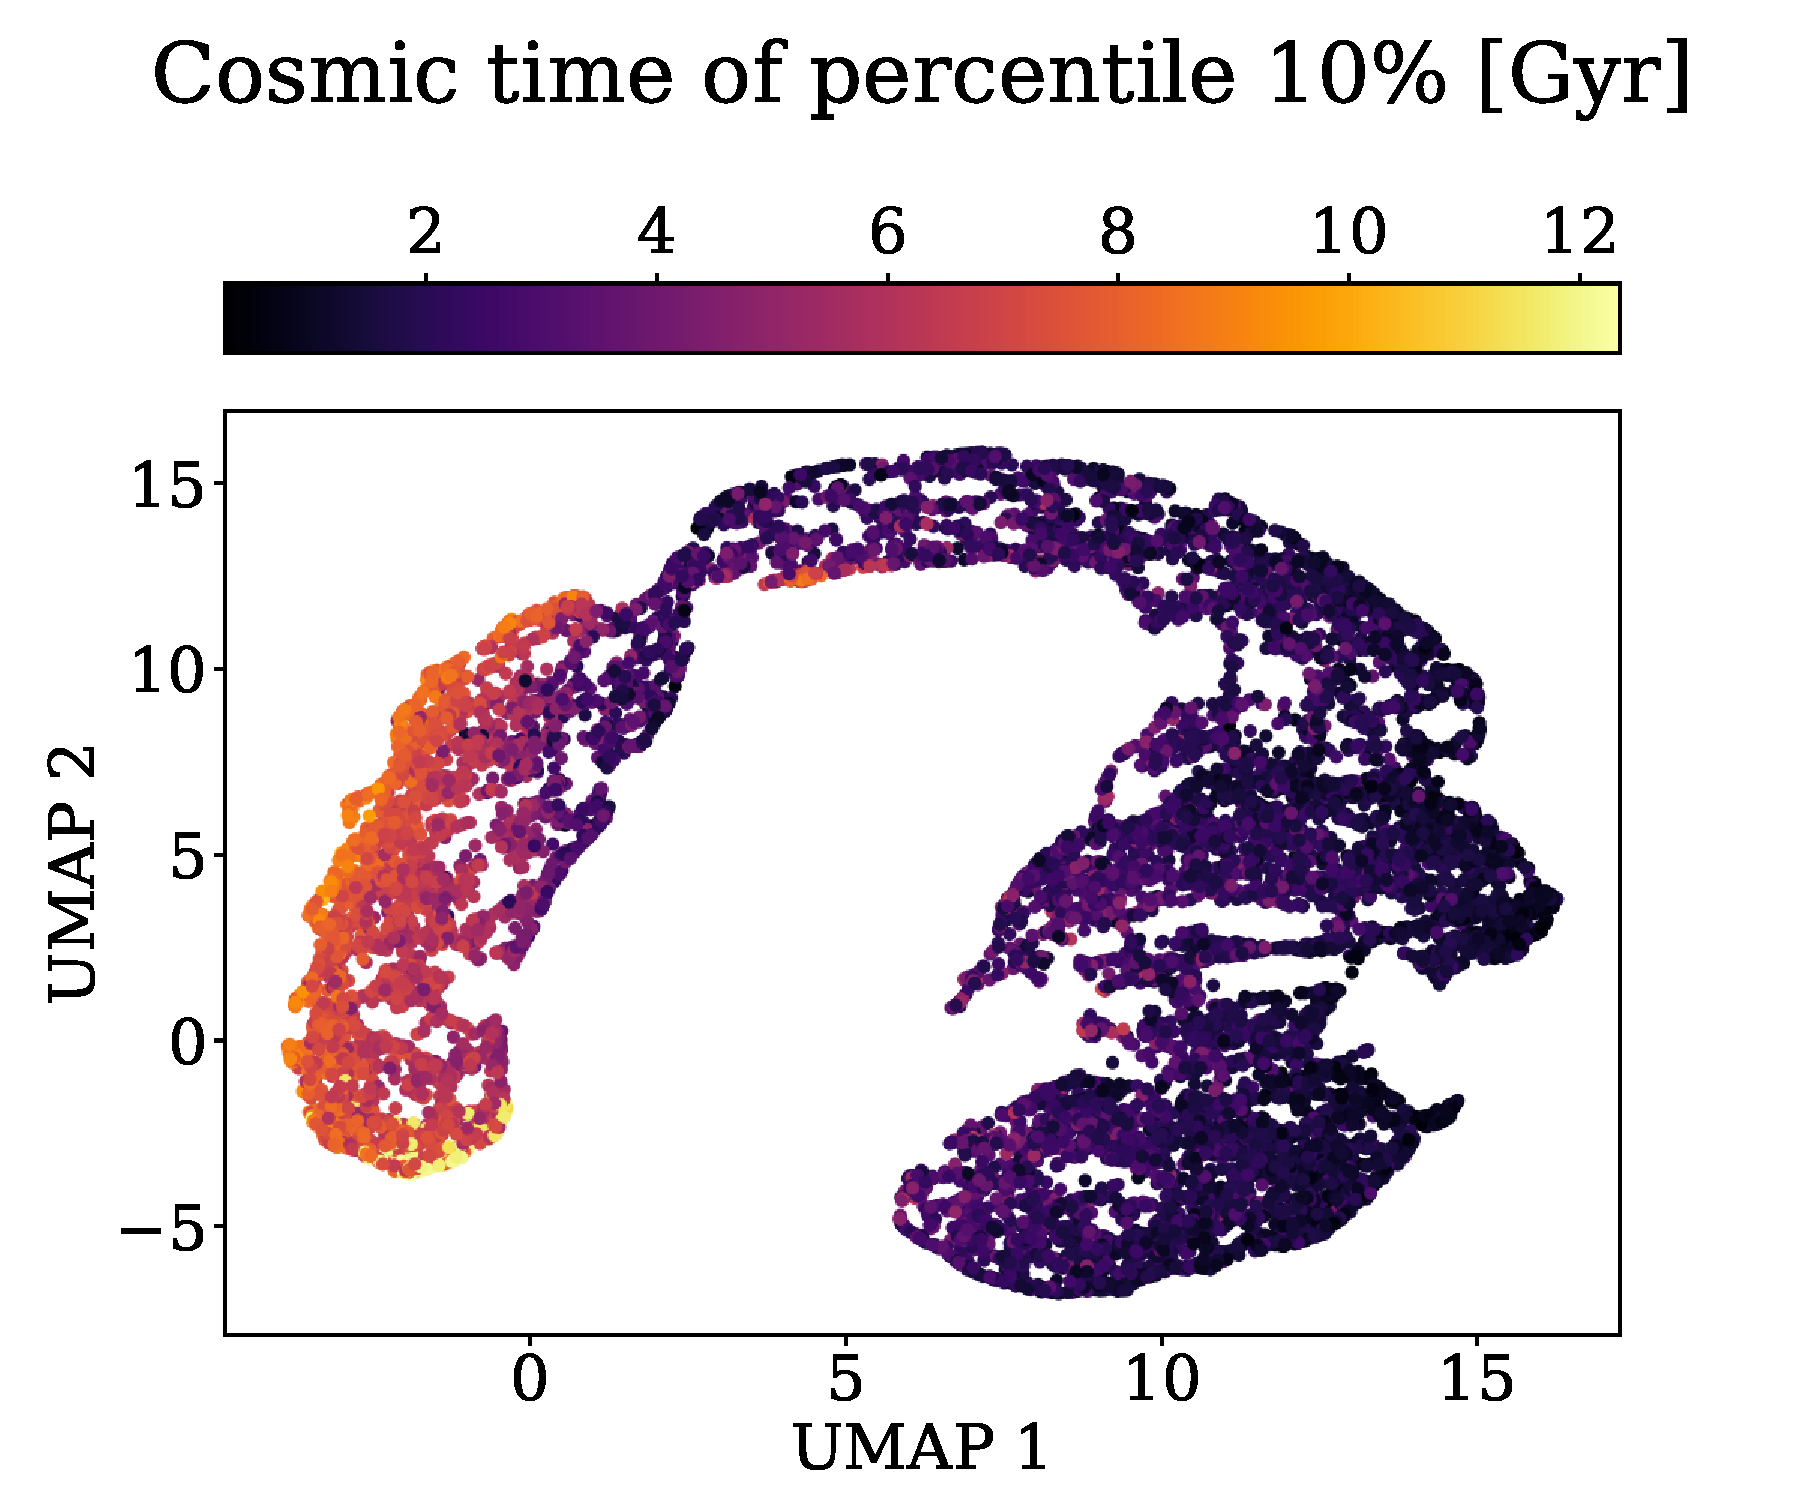
\includegraphics[width=0.33\textwidth]{images/latents/UMAP_10.pdf}
    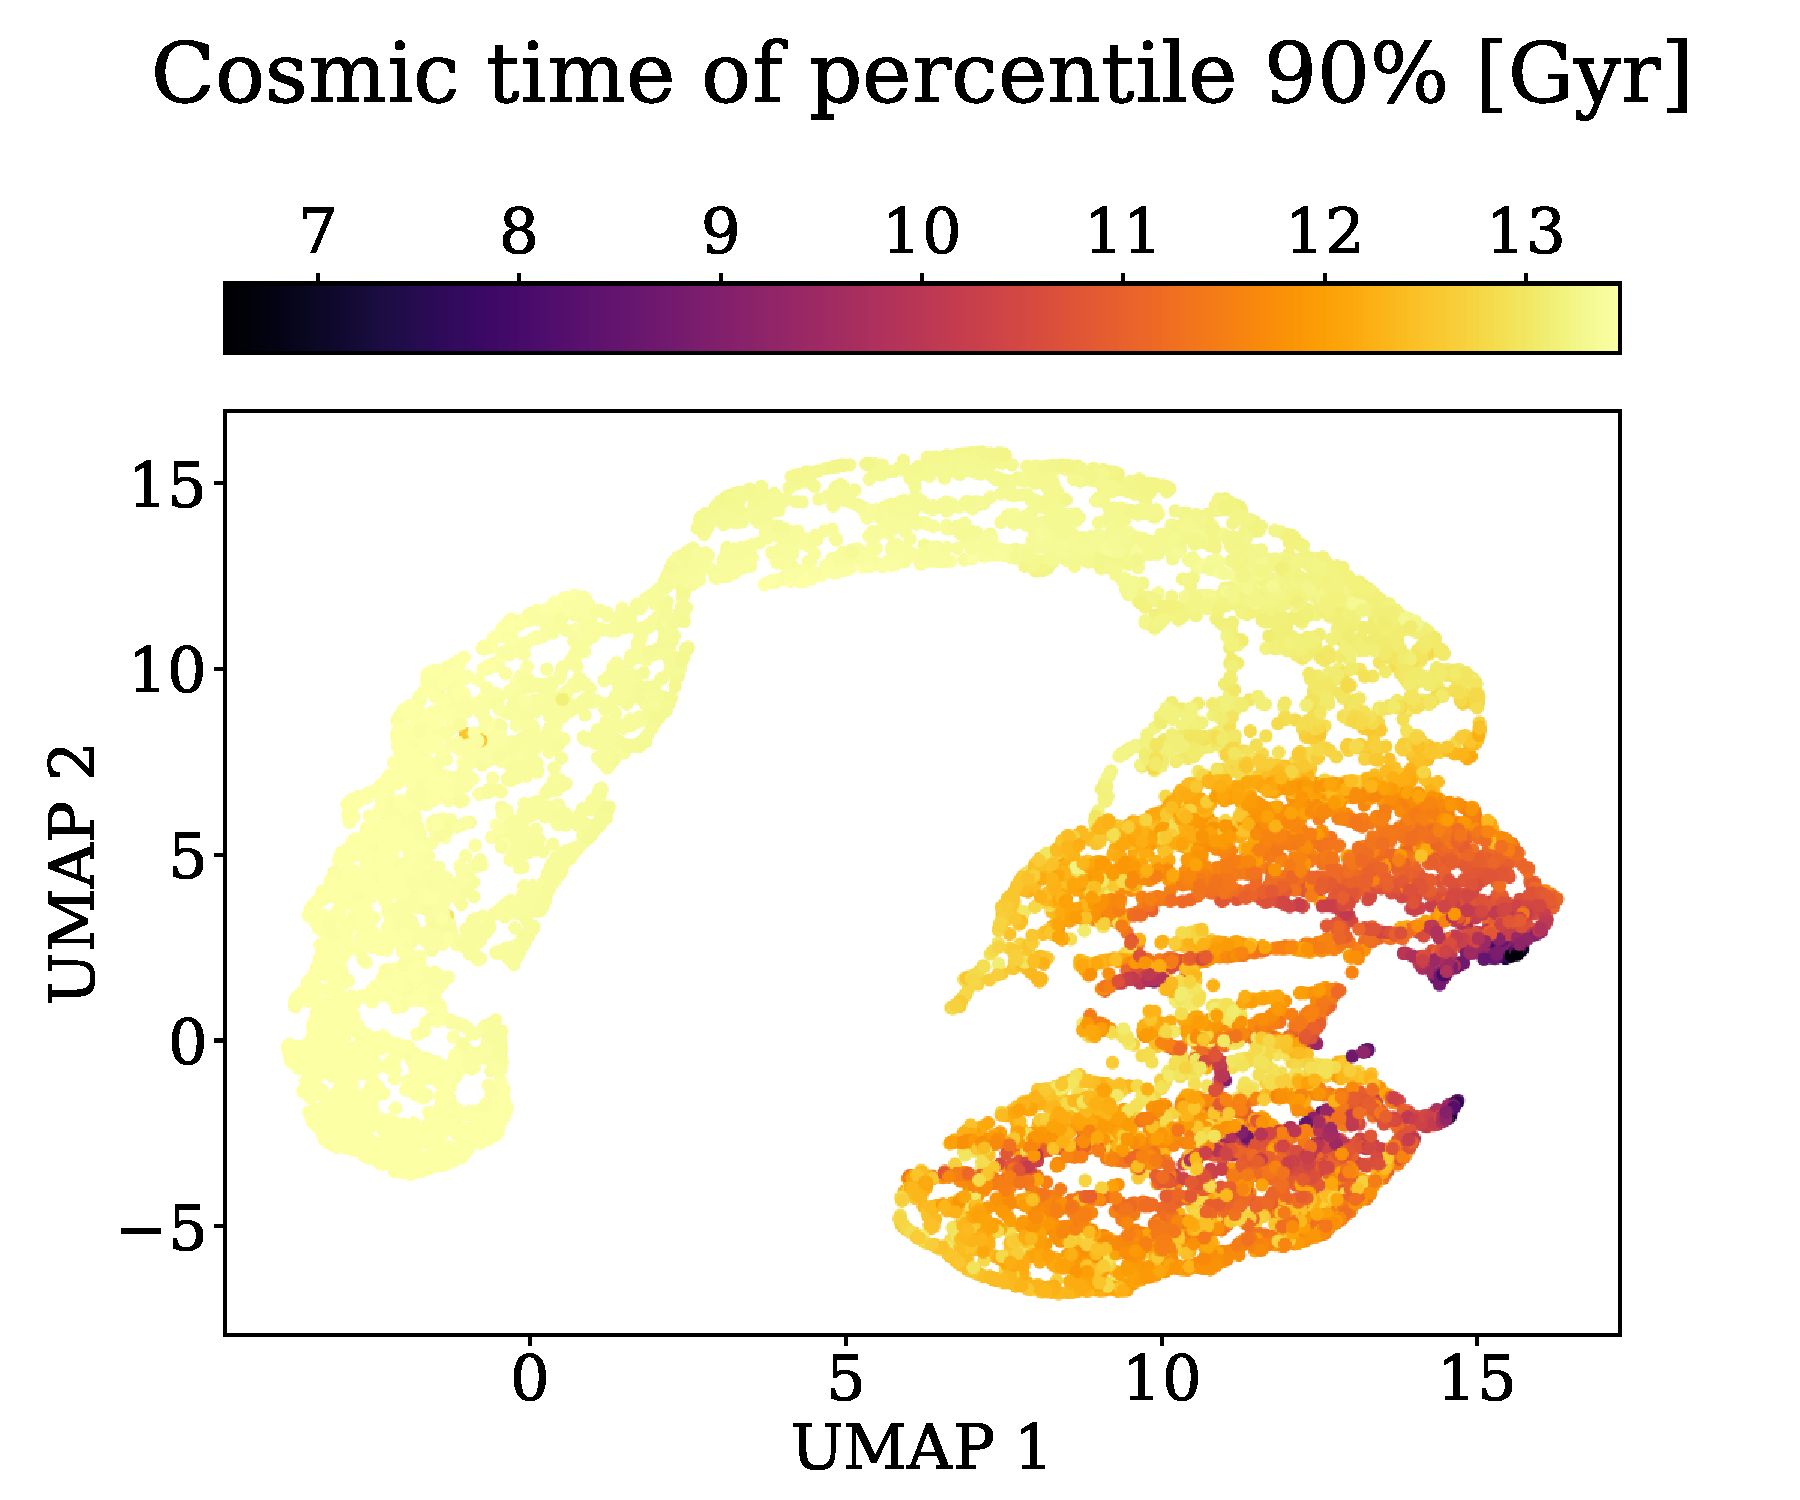
\includegraphics[width=0.33\textwidth]{images/latents/UMAP_90.pdf}
    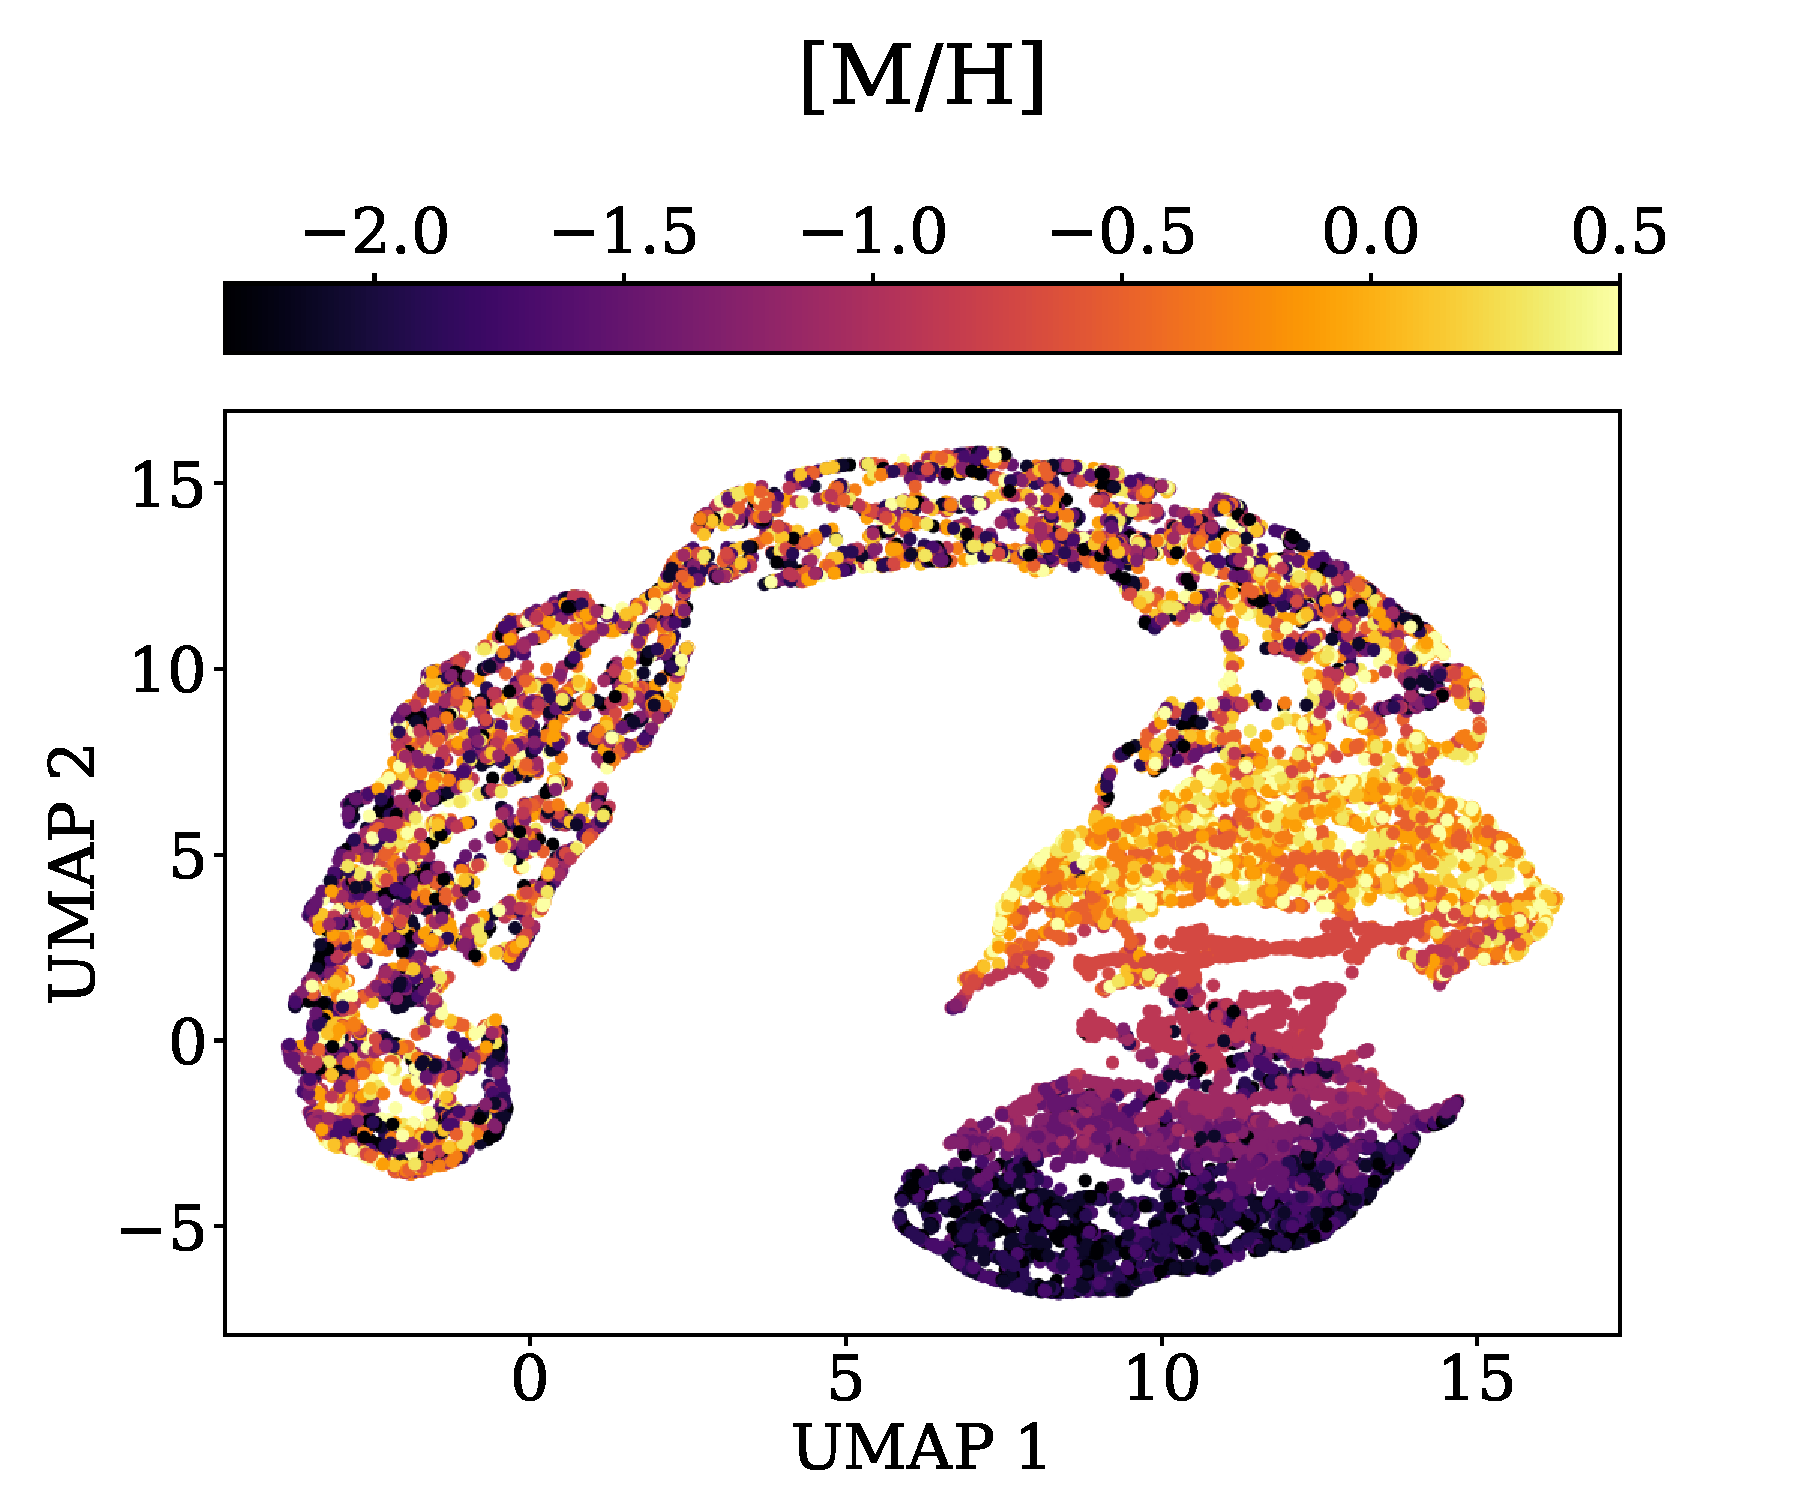
\includegraphics[width=0.33\textwidth]{images/latents/UMAP_met.pdf}
    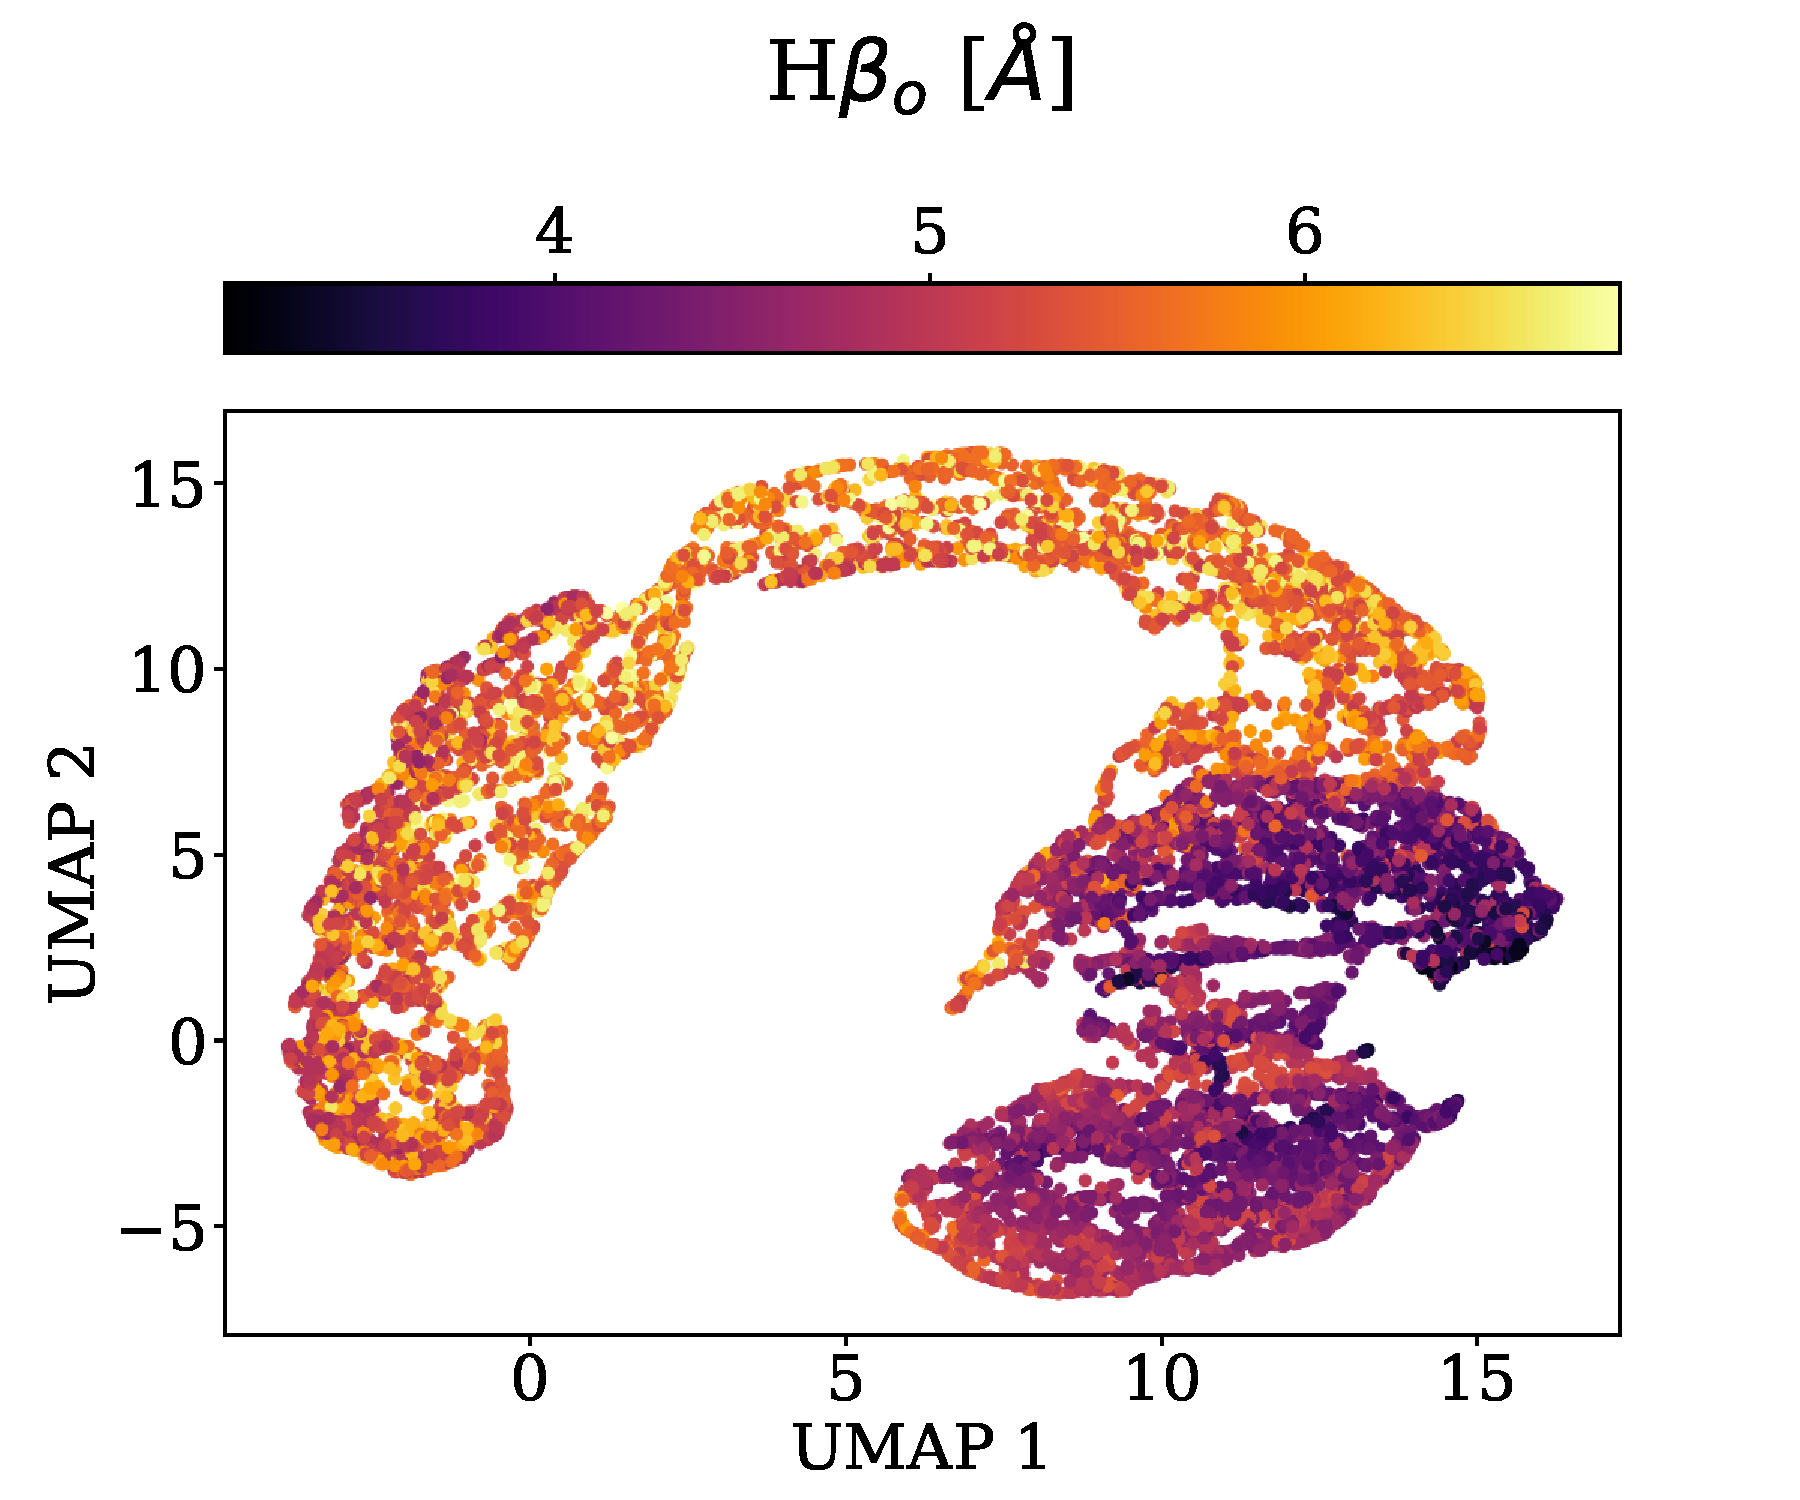
\includegraphics[width=0.33\textwidth]{images/latents/UMAP_hbeta.pdf}
     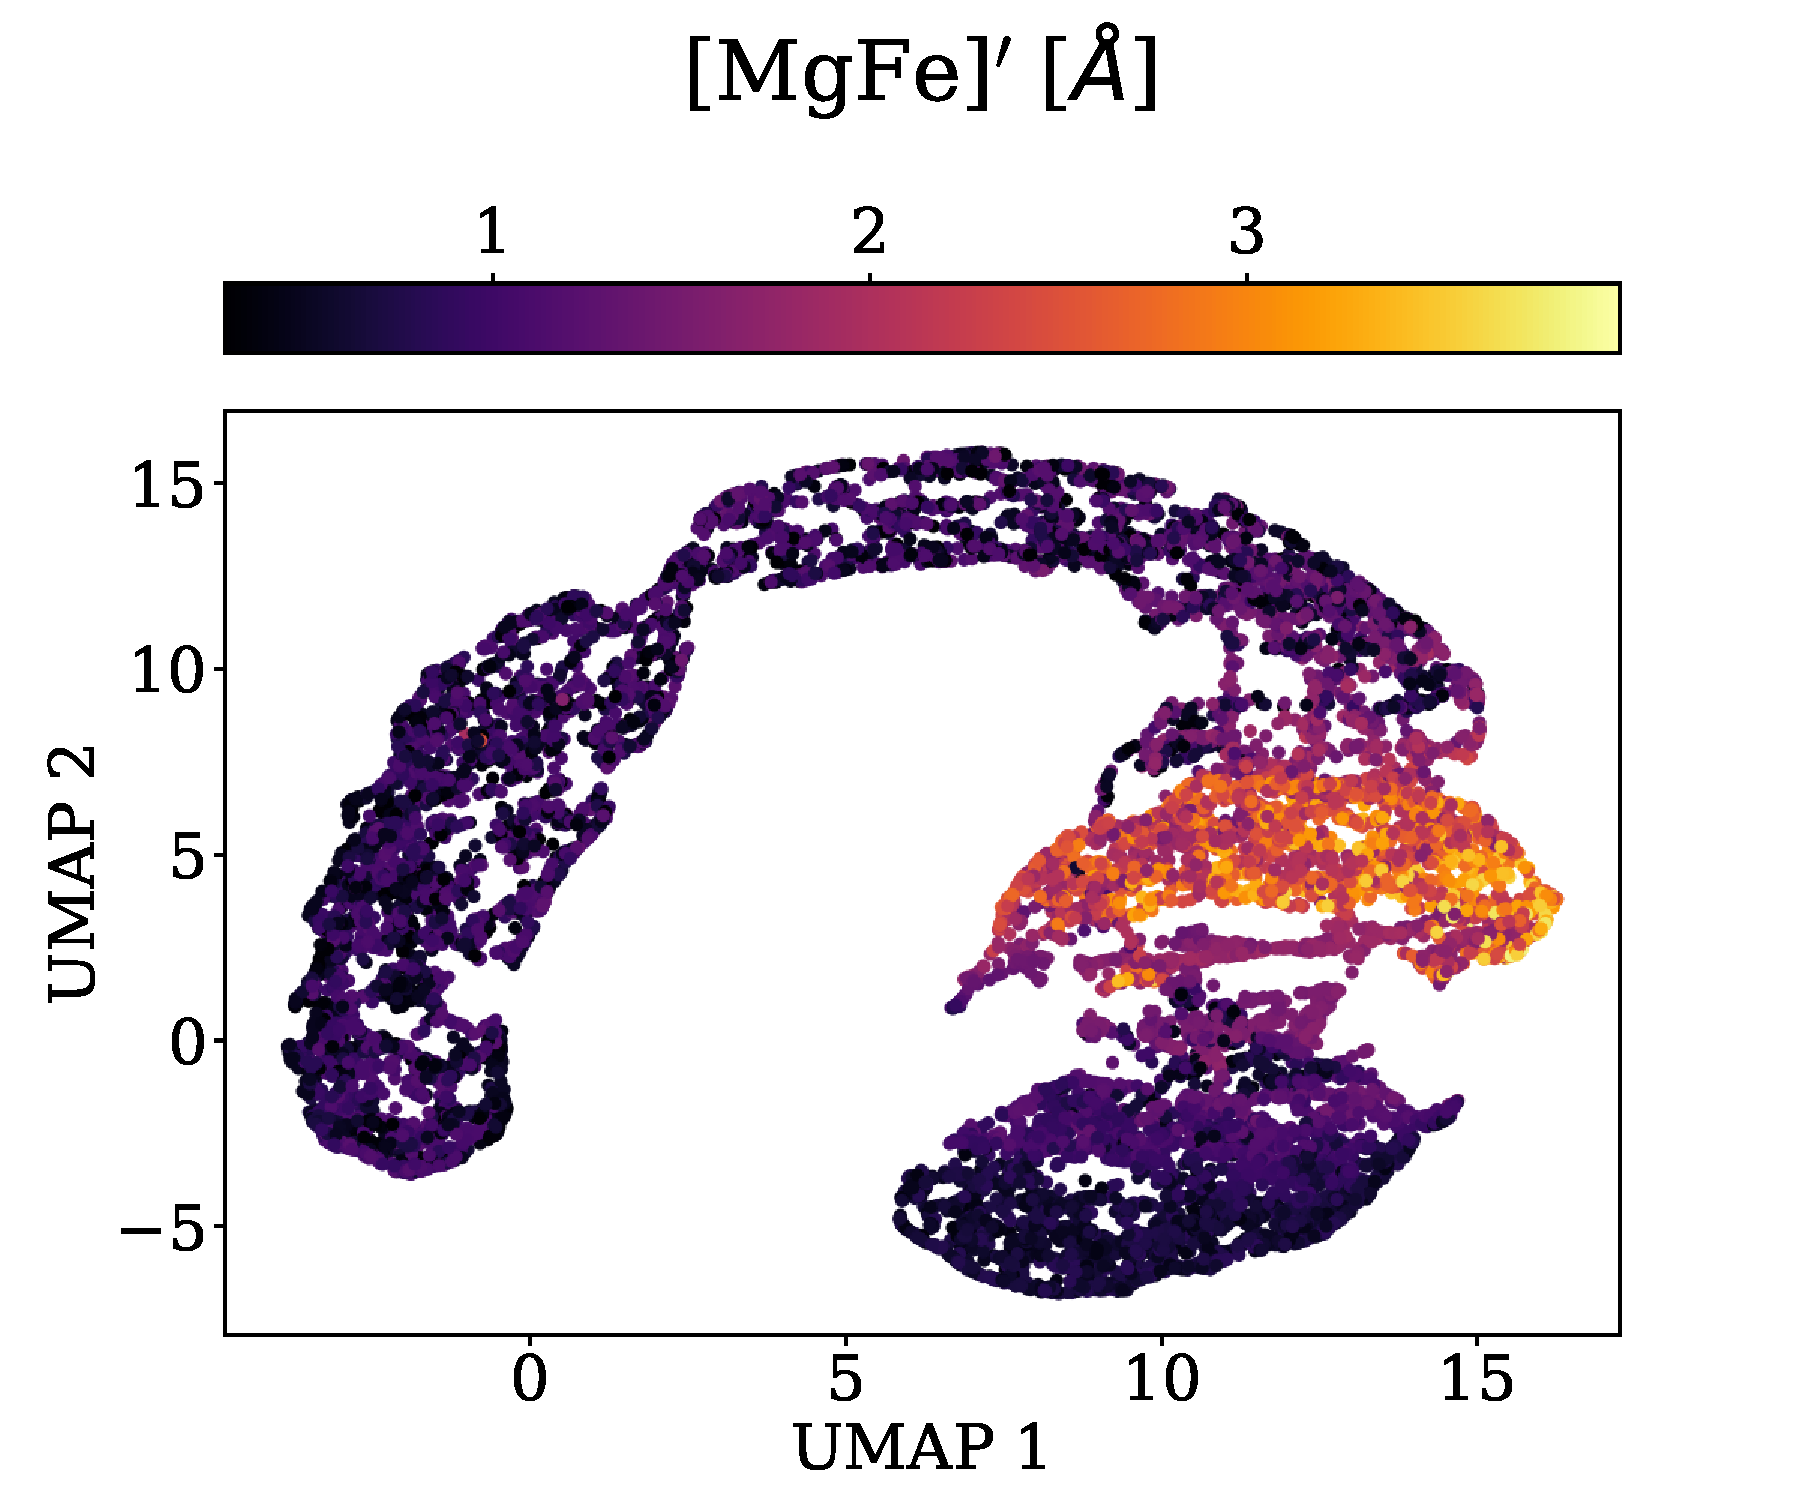
\includegraphics[width=0.33\textwidth]{images/latents/UMAP_mgfe.pdf}


     
    \caption{UMAP embedding for the latent representations. Each dot corresponds to a synthetic galaxy from the test sample. The closer two galaxies are on the map, the more similar are their latent representations. Different colourmaps are set according to the cosmic time at which the percentiles $10\%$ (top left) and $90\%$ (top middle) of the total stellar mass are reached, $[\rm{M/H}]$ (top right), and the two line indices  $\rm H{\beta_{o}}$ (lower left) and $[\rm{MgFe}]^{\prime}$ (lower right). Clear trends can be observed, demonstrating that the information encoded in the latent vectors is optimal for recovering the SFHs and metallicities.}
    \label{umap}
\end{figure*}



\subsection{Recovering SFHs of synthetic galaxies}
\label{post}
The network is trained with $90$\% of the generated samples ($x=$ {latent vectors}, $y=$ {nine stellar mass percentiles, $\rm{[M/H]}$}), with $10\%$ of these composing the validation set. Once the training is finished ($\sim4$ hours: $1$ hour for the encoder and $3$ hours for the Normalising Flows), the remaining $10$\% of the samples is used to test its performance, by obtaining probability distributions for the values of each percentile and $\rm{[M/H]}$ from their latent representations, and comparing the distributions with the true values. Each posterior estimation for the test set is performed with $1{,}000$ samples, taking $\sim0.4$\,s to get the predictions for the $10$ quantities of each galaxy. All the time estimations have been made using a NVIDIA Tesla P100 PCIe GPU with 12GB.\\



Figure \ref{examples} shows five examples of synthetic SFHs from the test set. The true values for the mass percentiles are indicated with  solid lines, while the recovered median of the posterior is shown with dashed lines. Light- and dark-shaded areas indicate the one and two $\sigma$ confidence intervals. It its clear that the model can recover from the latent vectors SFHs that are fully consistent with the ground truth within the expected uncertainties. In Fig.~\ref{meanvstrue}, we plot the median values of the posterior distributions predicted for the $15{,}000$ test galaxies against the true values, for the percentiles $10\%$, $50\%$, $90\%$ (in cosmic time), and for the metallicity. Both agree, close to the one-to-one relation, reaching high $R^{2}$ values\footnote{Also known as coefficient of determination $\displaystyle R^2=1-\frac{\sum_{i=1}^n\left(y_i-\widehat{y}_i\right)^2}{\sum_{i=1}^n\left(y_i-\overline{y_i}\right)^2}$, not to be confused with the square of the Pearson's coefficient.} of $0.88$, $0.97$, $0.98$, and $0.96$, respectively.  A larger scatter is observed for earlier percentiles, which is expected as the luminosity of young stars `outshines' the spectra, hiding the information of the oldest ones. \\

Posterior distributions for the percentiles $10\%$, $50\%$, $90\%$, and for the metallicity are shown as a corner plot in Fig.~\ref{corner}, for a single galaxy from the test set. The posteriors have been sampled with $1{,}000$ realisations. They deviate slightly from Gaussian functions, showing multimodalities associated with the degeneracy between the age (in particular the percentile $90\%$)  and  the metallicity, but in perfect agreement with the true values, indicated with solid lines.\\


Figures \ref{examples}, \ref{meanvstrue} and \ref{corner} confirm that the model is indeed capable of recovering the stellar mass growth and metallicity with uncertainties associated with the complexity of the inversion problem, due to the very nature of the spectra and to the observational imprints left by galaxies on them.  \\



\begin{figure}[t]
    \centering
    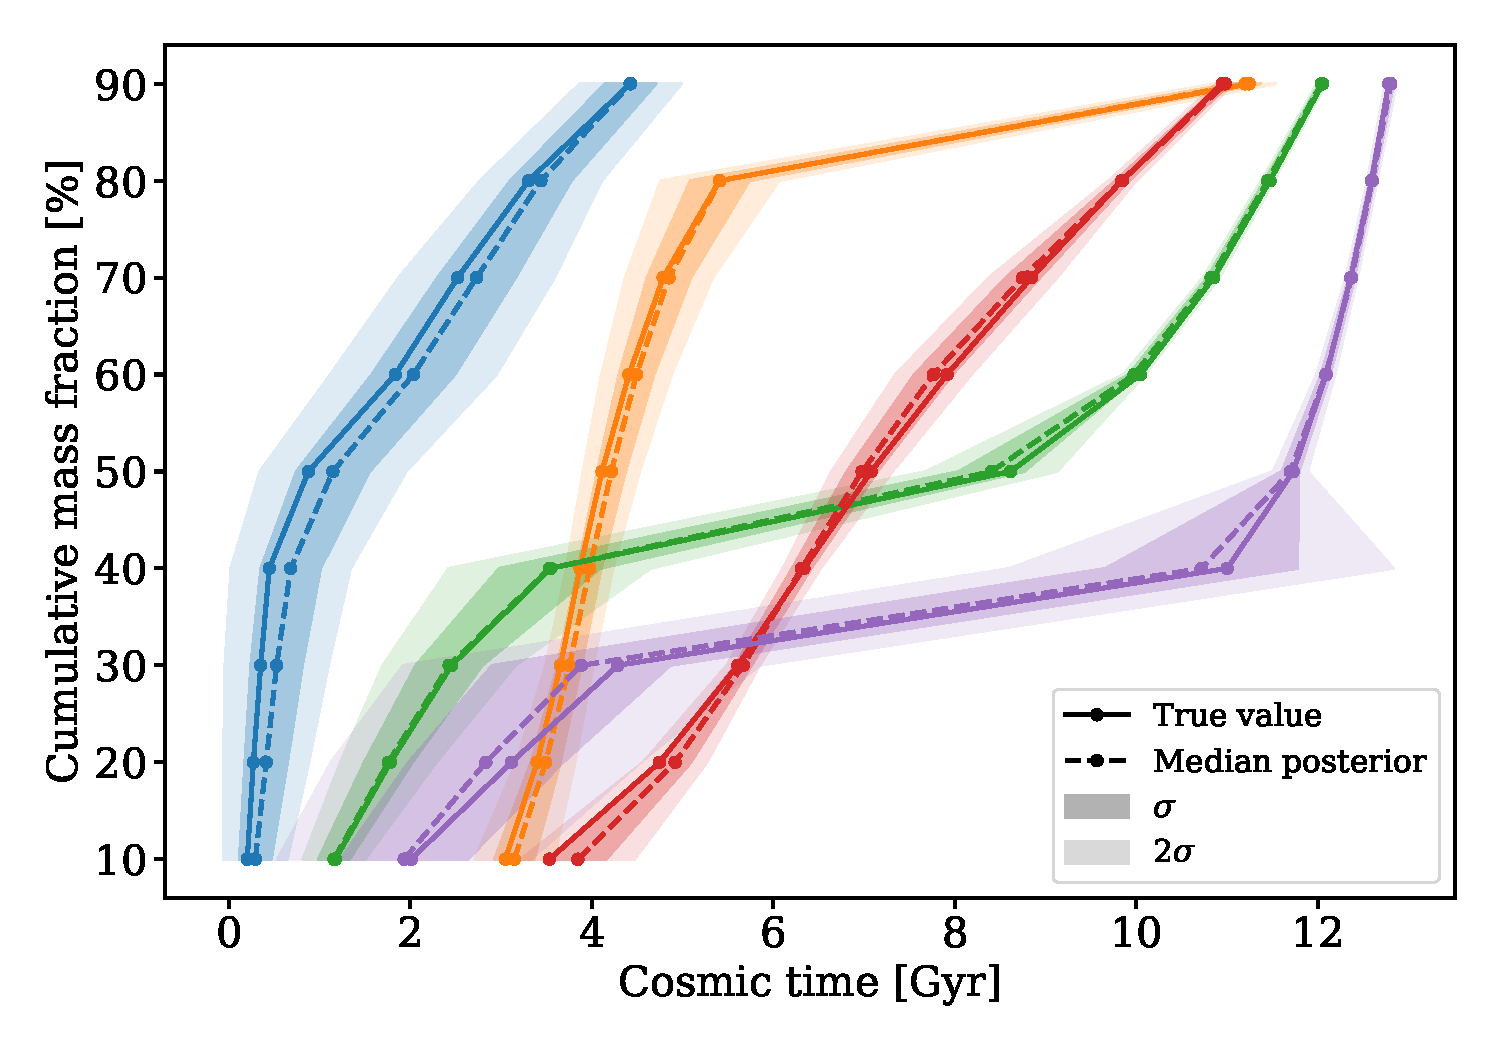
\includegraphics[width=0.49\textwidth]{images/posterior/cummul_mass_growth_2.pdf}
    \caption{Percentile predictions for five synthetic galaxies. The cumulative mass curves indicate the time at which the nine stellar mass percentiles are achieved over cosmic time. The solid lines correspond to the true values and the dashed ones to the predictions (medians of the posterior distributions). The $\sigma$ and $2 \sigma$ intervals of confidence are shaded dark and light, respectively. The model performs reliable reconstructions for all five galaxies.}
    \label{examples}
\end{figure}

\begin{figure}[h!]
    \centering
    
    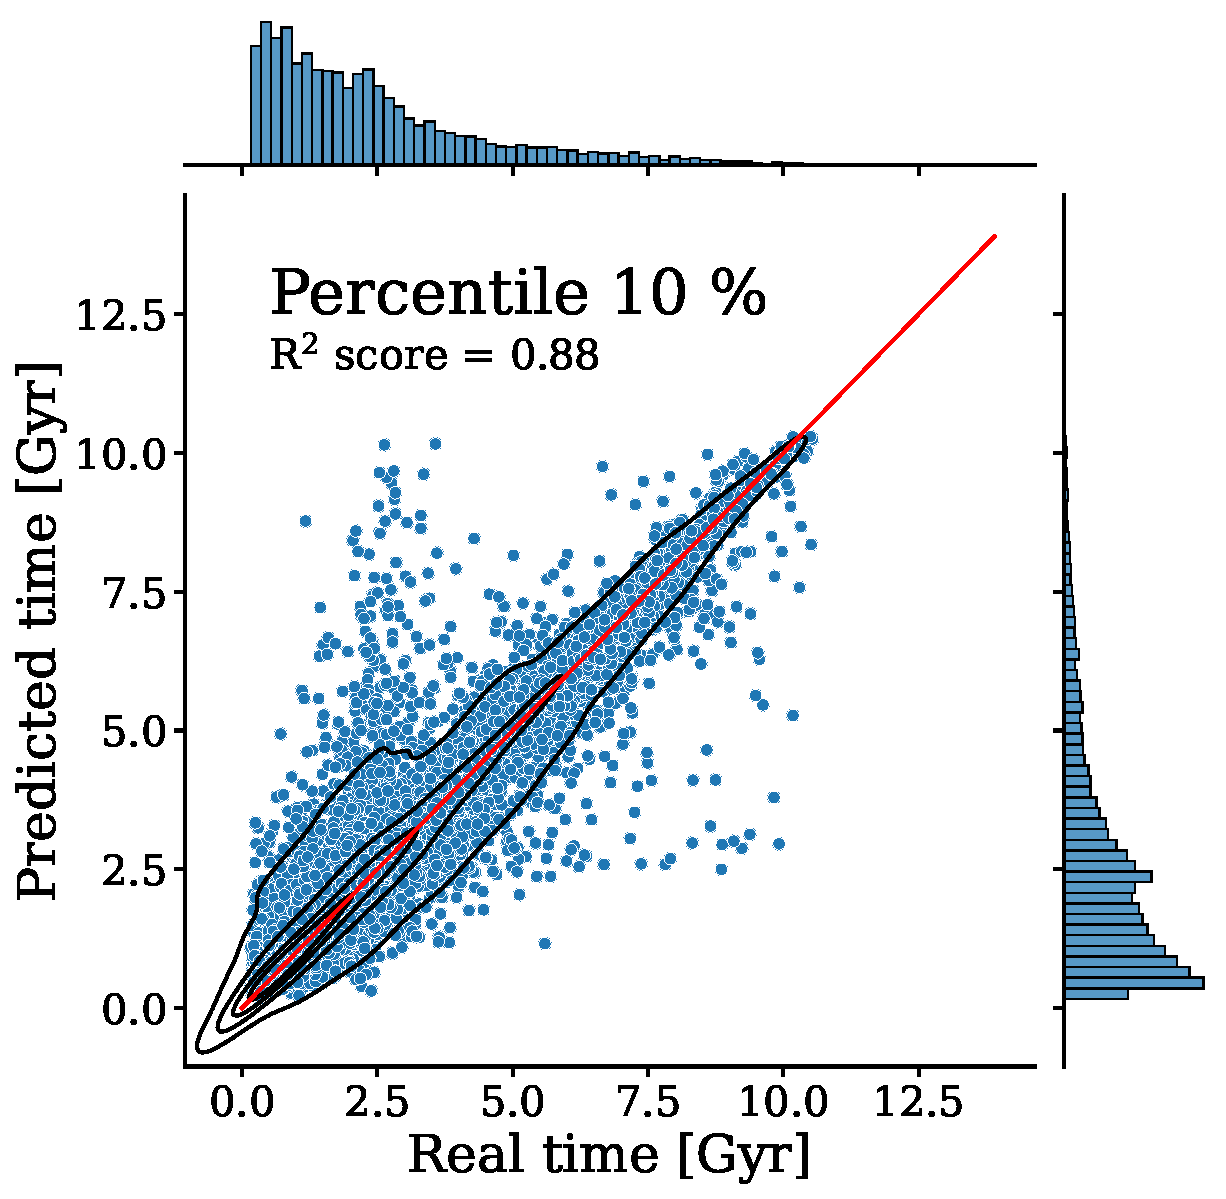
\includegraphics[width=0.285\textwidth]{images/posterior/sns_mean_true_0.pdf}
    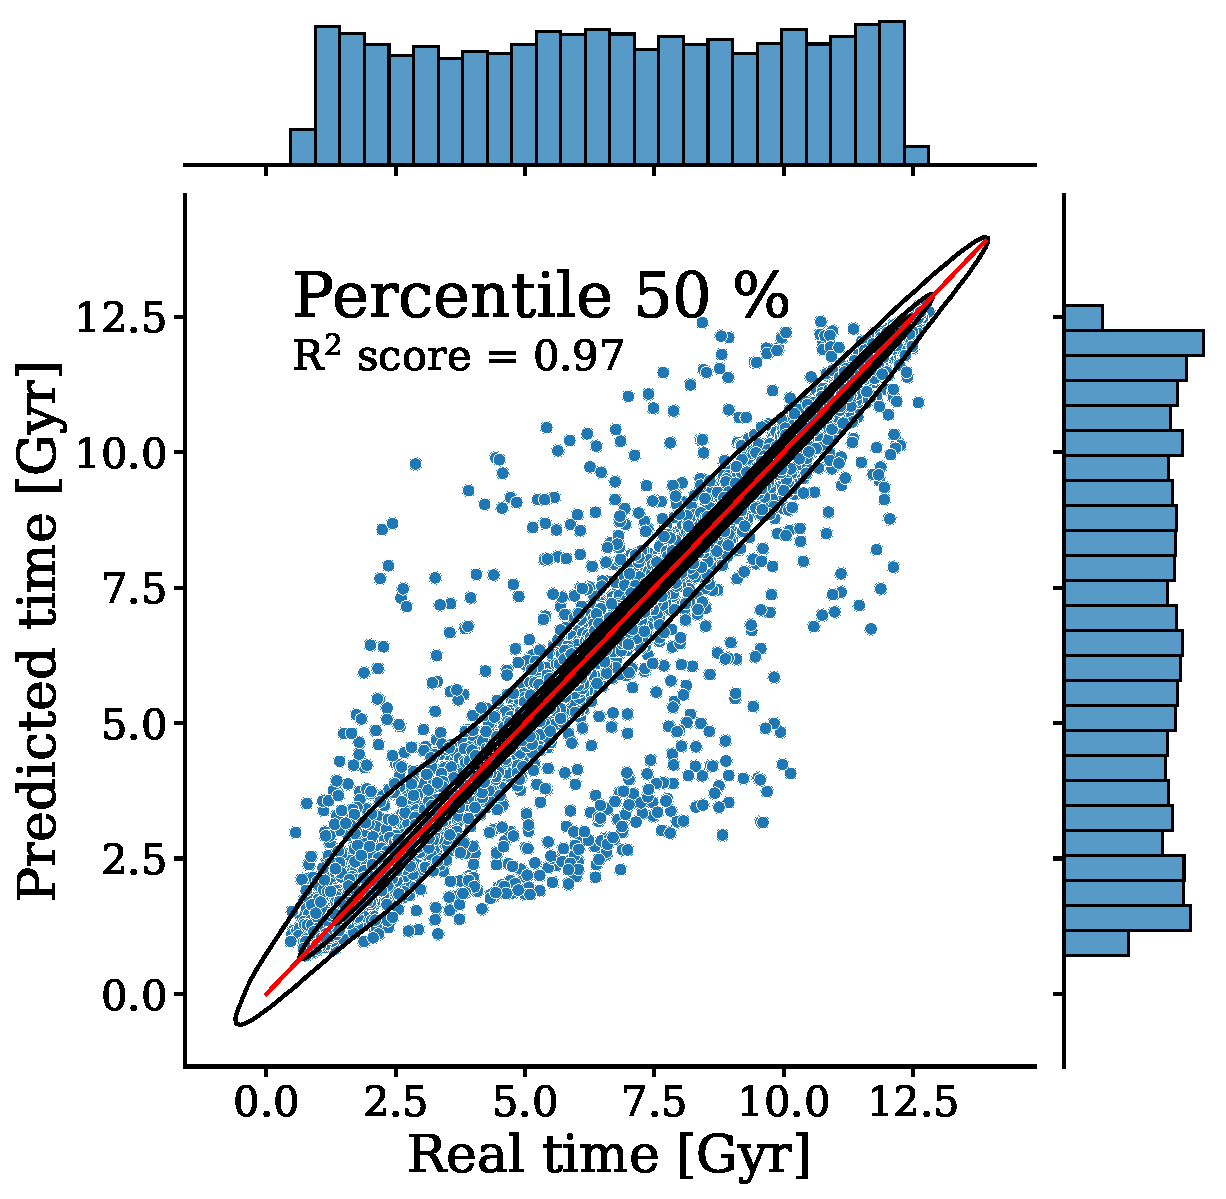
\includegraphics[width=0.285\textwidth]{images/posterior/sns_mean_true_4.pdf}
    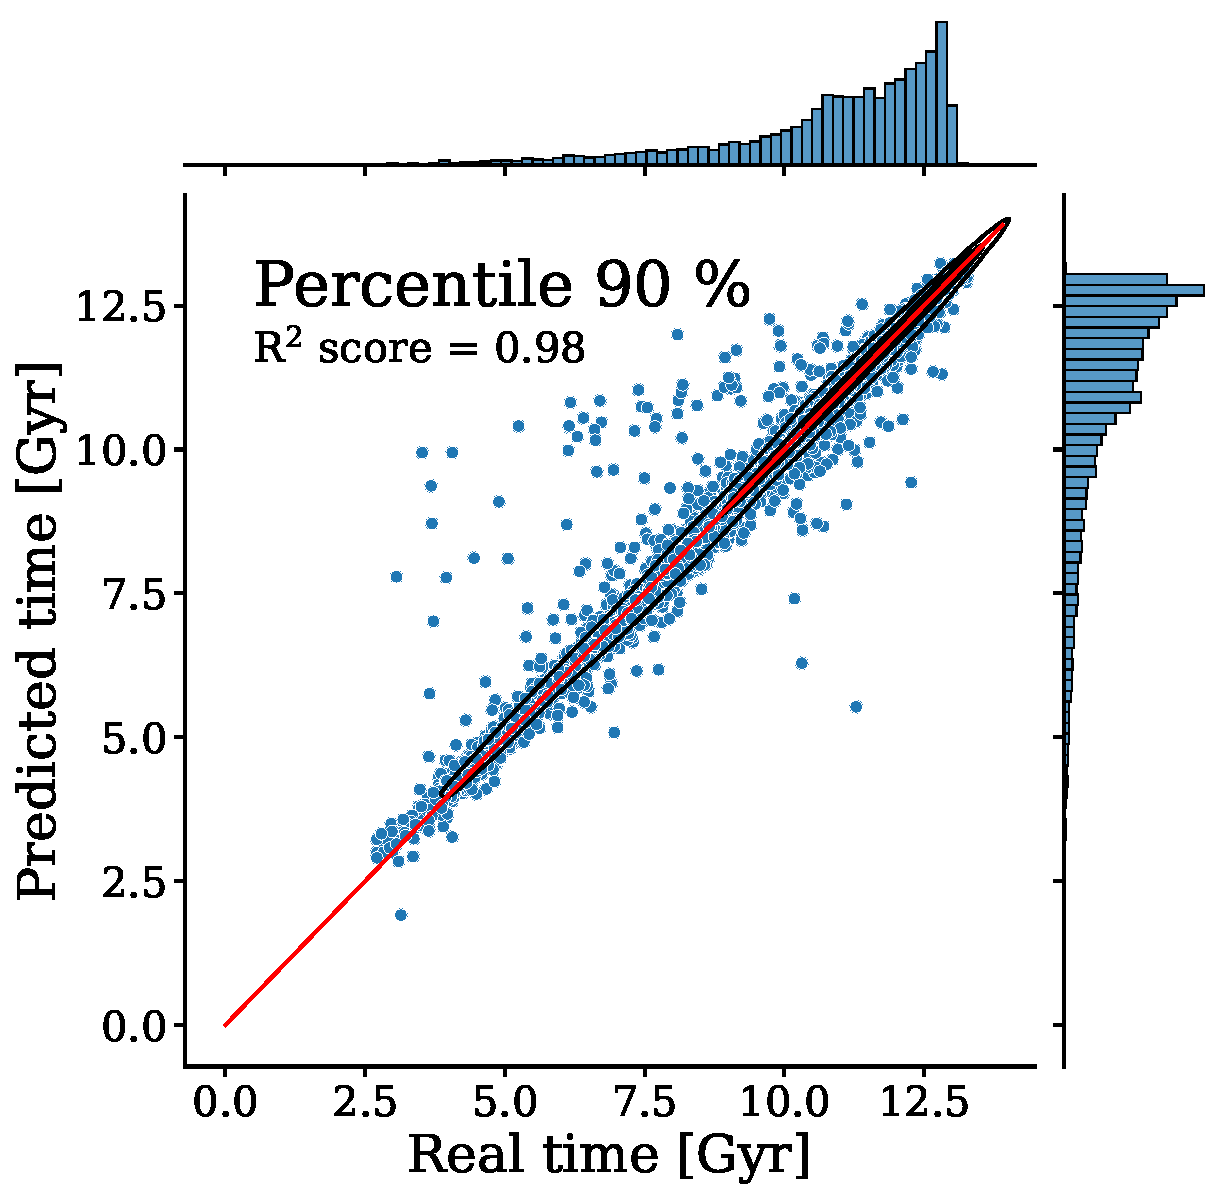
\includegraphics[width=0.285\textwidth]{images/posterior/sns_mean_true_8.pdf}
    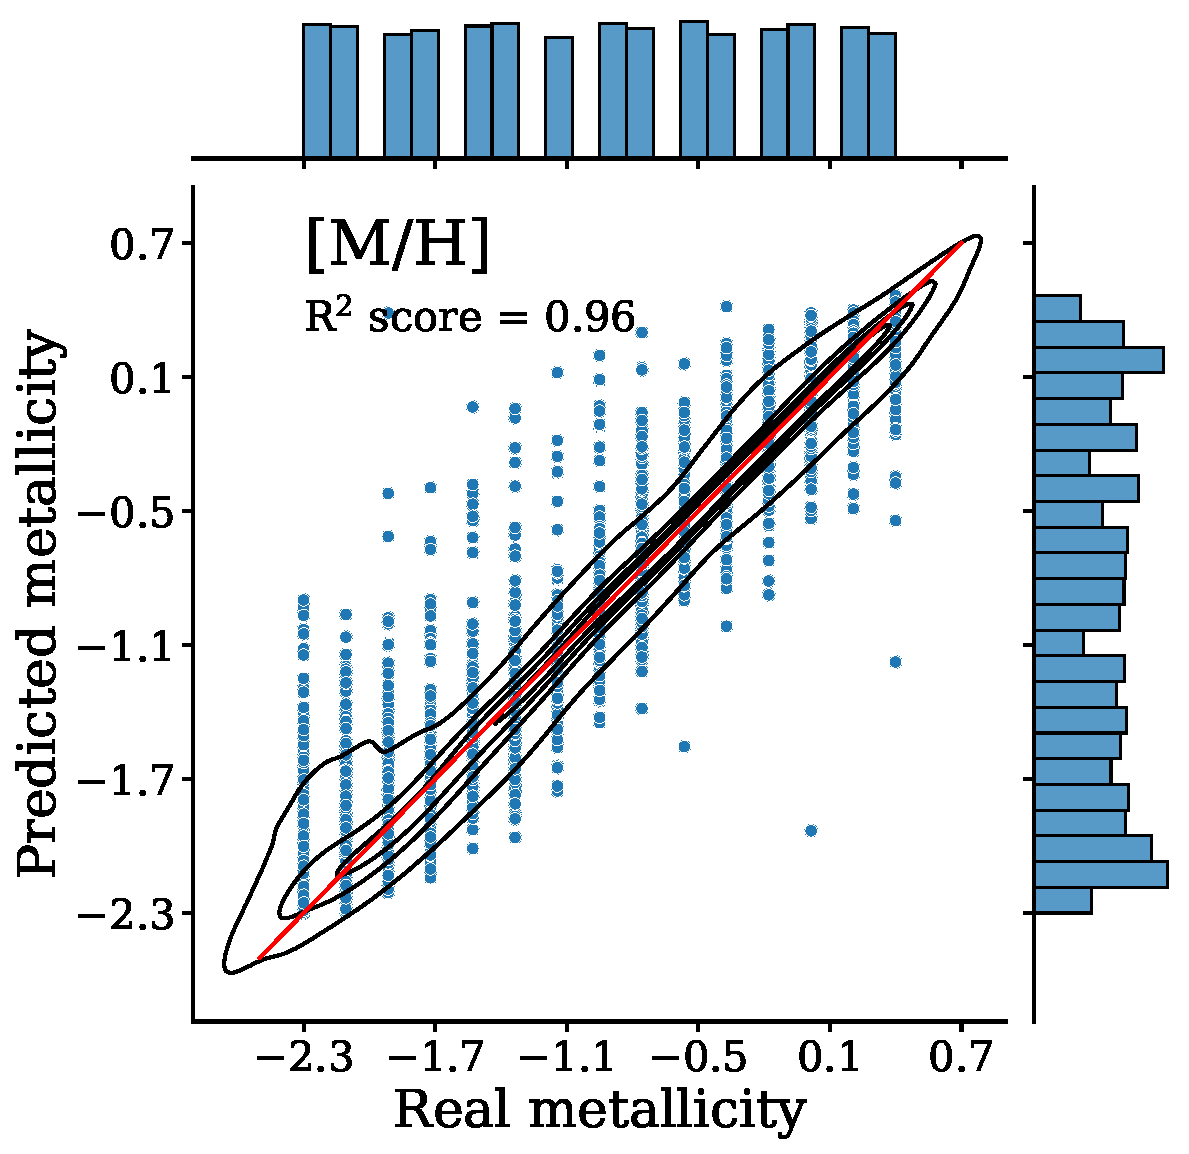
\includegraphics[width=0.285\textwidth]{images/posterior/sns_mean_true_9.pdf}
    
    \caption{Median values of the posterior distributions estimated for the percentiles $10\%$, $50\%$, $90\%$, and $\rm{[M/H]}$, compared to the true values. The $R^2$ score achieved for each prediction is $0.88$, $0.97$, $0.98$, and $0.96$, respectively. Each blue dot is a different sample from the test set. The red line shows the one-to-one relation, the histograms at the right of each panel show the marginal distributions of the predictions, and the histograms of the real data are shown at the top. Kernel Density Estimation (KDE)  contours are drawn in black at iso-proportions of the density of samples.}
    \label{meanvstrue}
\end{figure}



\begin{figure}[h!]
    \centering
    
    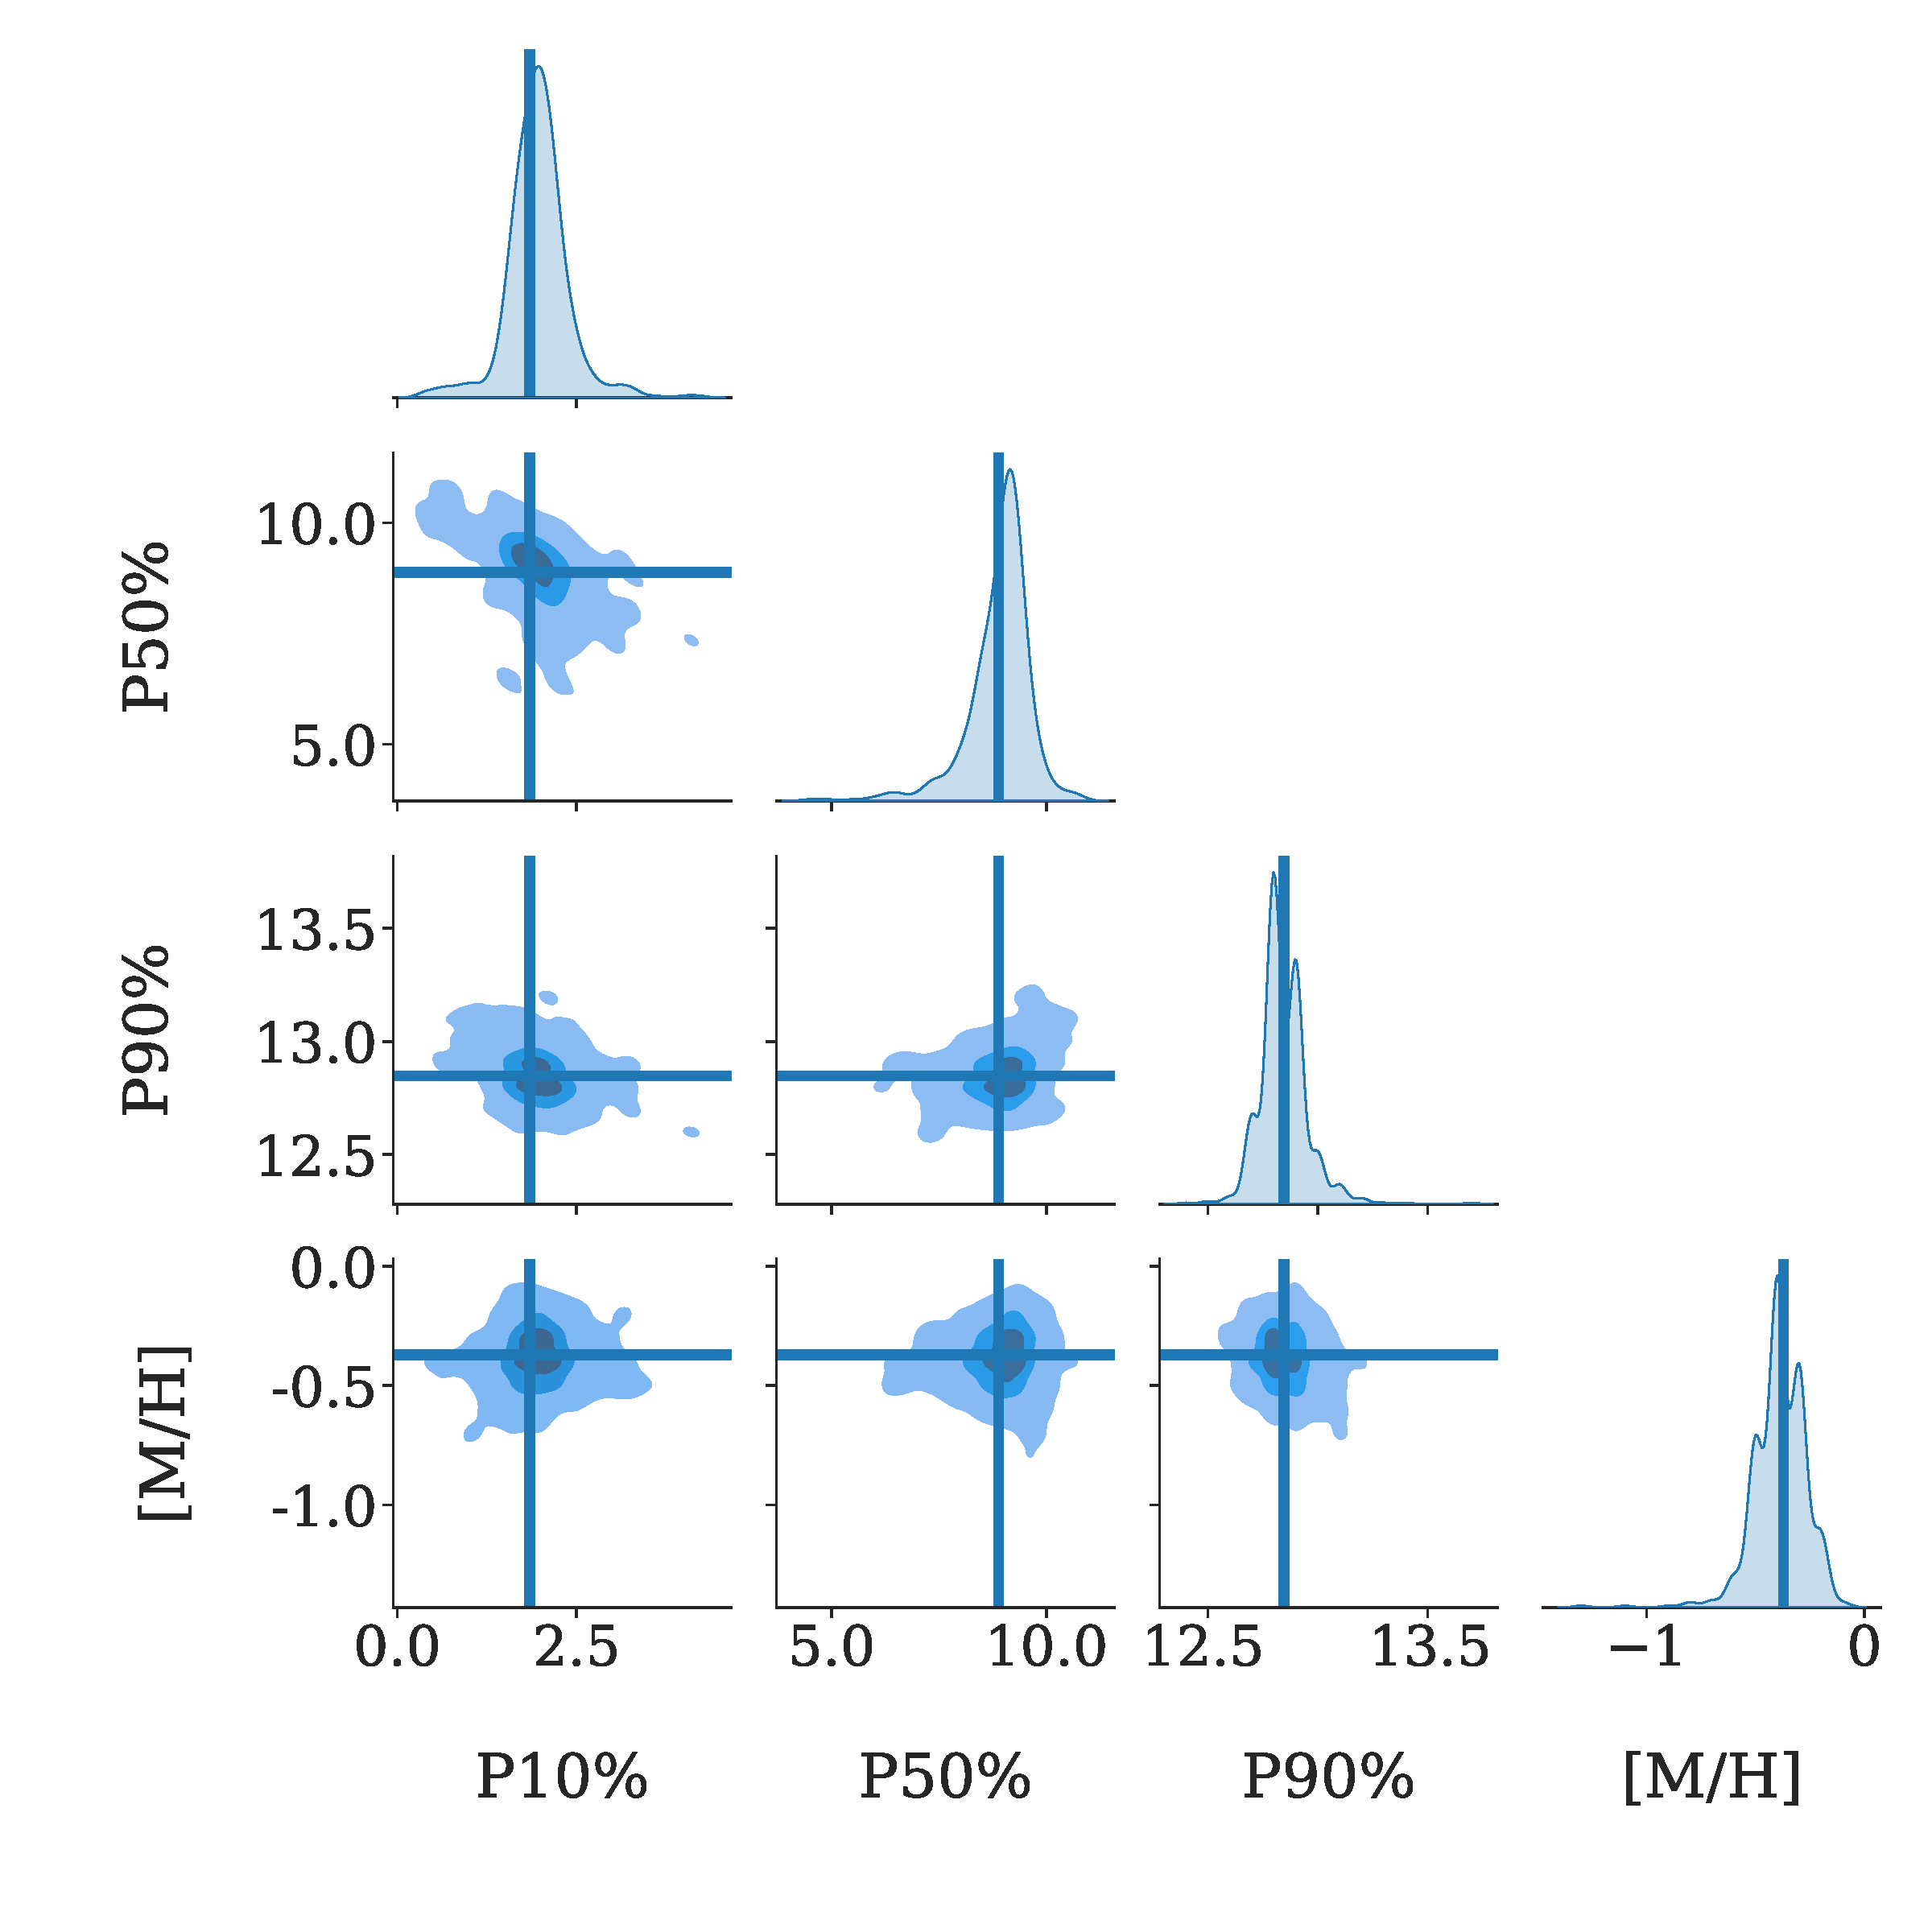
\includegraphics[width=0.5\textwidth]{images/posterior/conerplot0_ok.pdf}

    \caption{Corner plot with the posterior distributions for a simulated galaxy, sampled with $1{,}000$ realisations for the percentiles $10\%$, $50\%$, $90\%$, in Gyr, and for $\rm{[M/H]}$. KDE contours are drawn with different shades at iso-proportions of the density of samples. The solid lines correspond to the true values.  The distributions deviate slightly from Gaussian functions, showing  multimodalities associated with the degeneracy of the parameter space, but in perfect agreement with the true values. }
    \label{corner}
\end{figure}

\subsection{Simulation-based calibration}
\label{sbc}
A key point is ensuring that the estimated posterior distributions are well calibrated. We use simulation-based calibration (SBC) as described in  \cite{talts2020validating} to examine the distribution of the rank statistics of the true parameter values withing the marginalised posteriors, which must be uniform if the posterior samples are consistent with the prior. The only requirement of this test is that we have a generative model for our data, so that we are able to obtain observations from the predicted posteriors of the physical parameters. This is not exactly true in our case, since we obtain a SFH sampled with nine time bins (the percentiles) instead of $1{,}000$, as used during the forward model. For this reason, and with the only purpose of carrying out this test, we repeat the model training  with a simulation that only takes into consideration the percentiles, performing the linear combination with nine spectra, so that with the posteriors provided by the model we are able to recover directly the synthetic observations.\\

Figure \ref{ranks} shows a histogram from an ensemble of rank statistics of $1{,}000$ prior samples relative to the corresponding posterior samples,  for the percentiles $10\%$, $50\%$, $90\%$, and for $\rm{[M/H]}$. Each histogram is complemented with a grey band indicating $99\%$ of the variation expected from a uniform histogram. Additionally, in Fig.~\ref{ecdf} we include the empirical cumulative distribution function (CDF), together with the diagonal expected from a well-calibrated posterior. Both plots show uniformly distributed ranks, and consequently an optimal overall performance, except for the metallicity, where we detect a slight $\cap$ shape. This symmetric deviation, related with the wide binning of $\Delta\rm{[M/H]}=0.1929$ we use throughout the work\footnote{A finer binning is always possible, but at the cost of a larger training set and longer training time.}, implies that the computed posterior will be wider than the true posterior, allowing us to estimate an upper limit for the uncertainty of the parameter.






\subsection{Testing with observations}

\label{obs}

To test the method we compare our measurements for $18$  stacks of early-type galaxies at $z \sim 0$ from SDSS spectra (with velocity dispersion in the range $100-320$ km/s), whose stellar populations have been studied in detail in \cite{La_Barbera_2013}. We highlight that the main advantage of working with these stacks is their very high S/N, and the absence of emission features, important because no noise models or emission lines have been incorporated in the simulation.\\

First, we convolve all the observations to emulate the maximum velocity dispersion of the dataset. Then, we clip the wavelength range to $[4023,6000]$ $\AA$, the maximum window that is common to all stacks. We also process the MILES spectra used for training to simulate the conditions of the observations. Once all the artificial spectra have the same resolution and wavelength range as the observations, we repeat the training, and then test the model performance again, analysing the impact of these changes on the performance.\\

As a result of the processing, the $R^2$ score on the synthetic test set decreases to $0.72$, $0.95$ and $0.96$ for the estimation of the percentiles $10\%$, $50\%$ and $90\%$, respectively, and to $0.96$ for the metallicity. These losses in performance, mainly for the first percentiles, are a direct consequence of reducing the resolution in the spectral lines, and clipping the Balmer jump in the bluer region of the spectra.\\




We then apply the trained model to the spectra of the stacks, sampling the posteriors with $10{,}000$ evaluations. In Fig.~\ref{percentiles_obs_full}, we show the median values of the measured distributions for the mass percentiles, as a function of cosmic time and redshift\footnote{Assuming a Planck13 cosmology \citep{planck13}.}, using a colourmap based on the velocity dispersions. The most massive galaxies (highest velocity dispersions) build up their stellar masses more abruptly, up to 90\% of their total stellar mass $1$ Gyr after the Big Bang, while the growth of stellar mass is softened as we move to less massive ones.\\ 

For a more detailed analysis, the median values of the posterior predictions, together with their uncertainties given by one standard deviation, are included in Table~\ref{table_obs}, for all $18$ observations. The quantities shown are the times by which $10$\%, $50$\% and $90$\% of the total stellar mass have been formed, as well as the metallicity. We do not find a clear trend between the metallicity and the velocity dispersion, but the margin of uncertainty is too large to make any further assumptions, mainly due to the wide binning in $\rm{[M/H]}$ of $0.1929$\,dex for the simulated sample. This is consistent with the results of \cite{La_Barbera_2013}, who reported a variation of $\sim 0.2$\,dex in metallicity from the least massive to the most massive stack.\\




Finally, we carry out a spectral reconstruction with our model in Fig~\ref{spectra_obs}, for the stacks with velocity dispersion $105$, $205$ and $300$ km/s. This test is usually referred to as Posterior Predictive Check (PPC,  \citealp{talts2020validating}), and allows us to verify that our measurements are indeed compatible with the observed spectra. These observed and reconstructed spectra must be close to each other in the latent space, but a priori this proximity is not trivial in the wavelength space, since we do not minimise the differences with respect to the observed spectra as in more traditional approaches, but perform the Bayesian inference on the latent representations. Even so, it is the most direct way we have of determining the  reliability of the measurements, and we do it by performing a linear combination of nine SSP MILES spectra of ages obtained from the percentiles of stellar mass, and metallicity fixed and equal to the predicted value. According to the definition of the percentiles, all nine spectra are weighted with $1/9$. The results are very positive, showing mean residuals of  $1.7\%$ between the fit and the observations, averaging over all $18$  stacks and wavelengths. The uncertainties are propagated into the spectra, within the grey-shadowed stripe in Fig~\ref{spectra_obs} corresponding to the interval of two standard deviations.

\subsection{Comparison with existing codes}
%to complete
\label{compare_ppxf}

We include another reconstruction of the spectra in Fig~\ref{spectra_obs}, namely a linear combination of MILES templates of  $34$ different ages and $12$ different metallicities ($408$ templates in total), where the weights are given by pPXF \citep{ppxf}. For a fair comparison, we use the same wavelength range as before without any continuum correction. The average of the residuals between the observed spectra and the pPXF fitting is $1.5 \%$. The observed spectra, our reconstructions from the percentiles and the reconstructions made with the weights of pPXF are in close agreement, not only in the latent space, but also in the wavelength space. We find that our method generally fits the spectra as accurately as pPXF despite, again, not being designed to reproduce them.\\

 On the other hand, the pPXF fitting takes $\sim30$ s for each stack, and since it does not provide an uncertainty, this measurement would be equivalent to a realisation of the posteriors obtained with our model, which take $4 \cdot 10^{-4}$\,s per stack.  Thanks to this acceleration of five orders of magnitude, our model can easily produce $10^3$ or $10^4$ samples of the posteriors for each observation and thus, always under the assumptions of the simulation, obtain a proper calibration of the uncertainty.


%time and deal with uncertainties in pPXF




\begin{figure*}[h!]
    \centering
    
    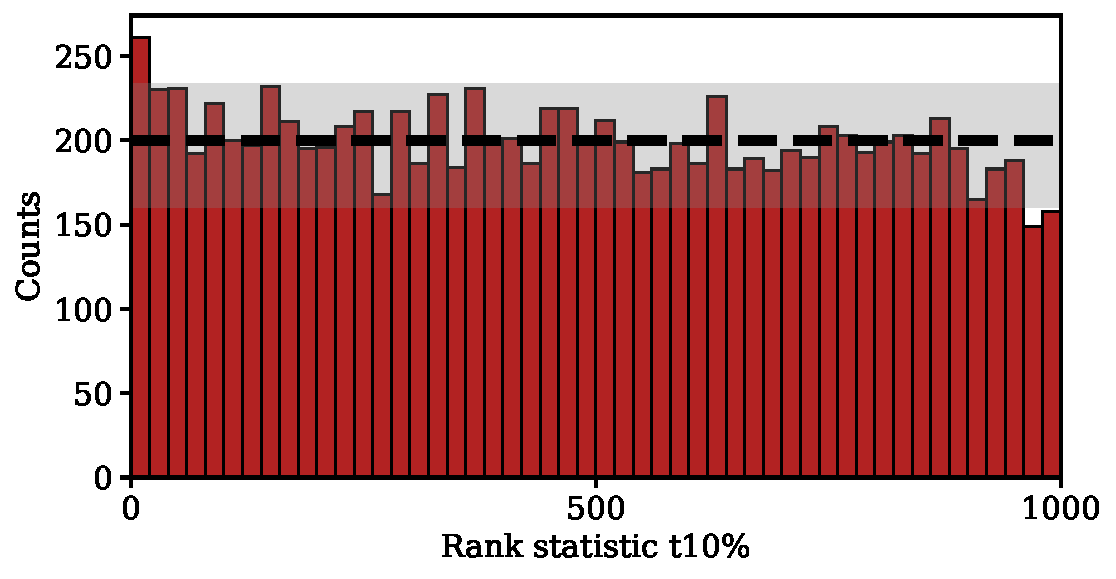
\includegraphics[width=0.45\textwidth]{images/sbc/rank_statisitic_1.pdf}
    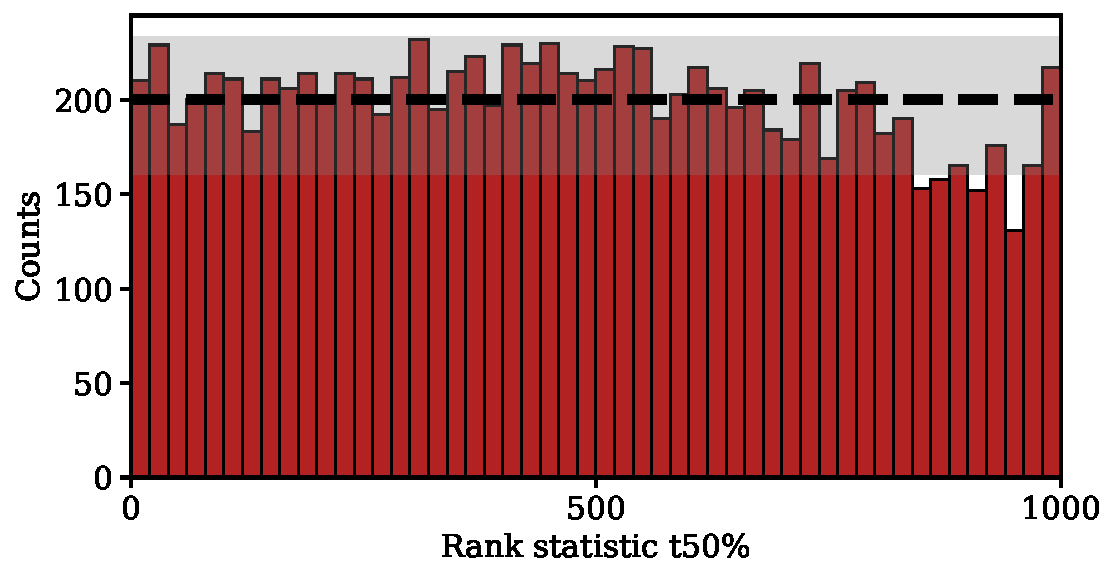
\includegraphics[width=0.45\textwidth]{images/sbc/rank_statisitic_2.pdf}
    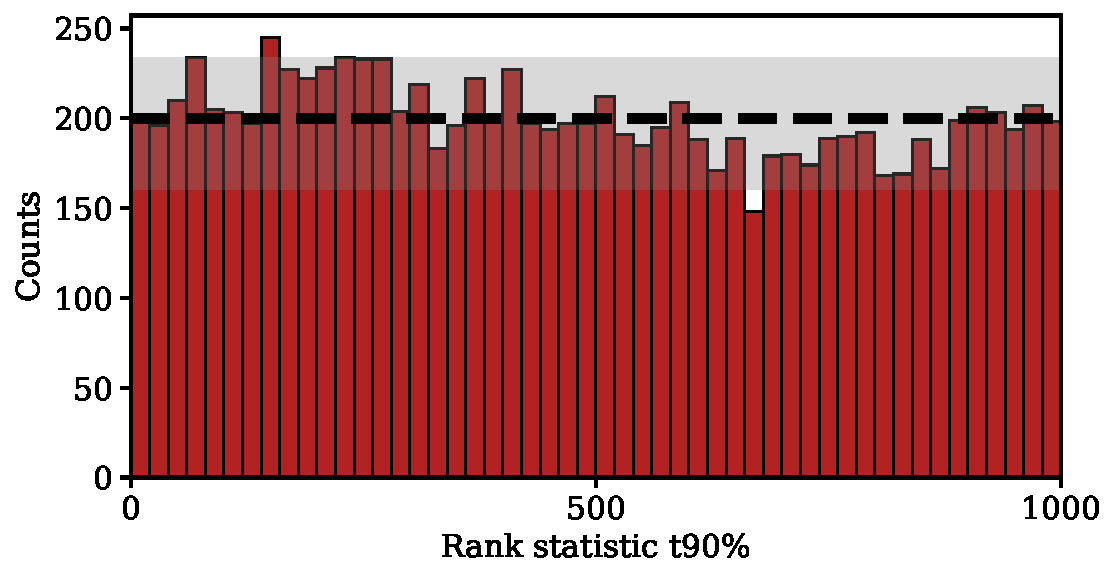
\includegraphics[width=0.45\textwidth]{images/sbc/rank_statisitic_3.pdf}
    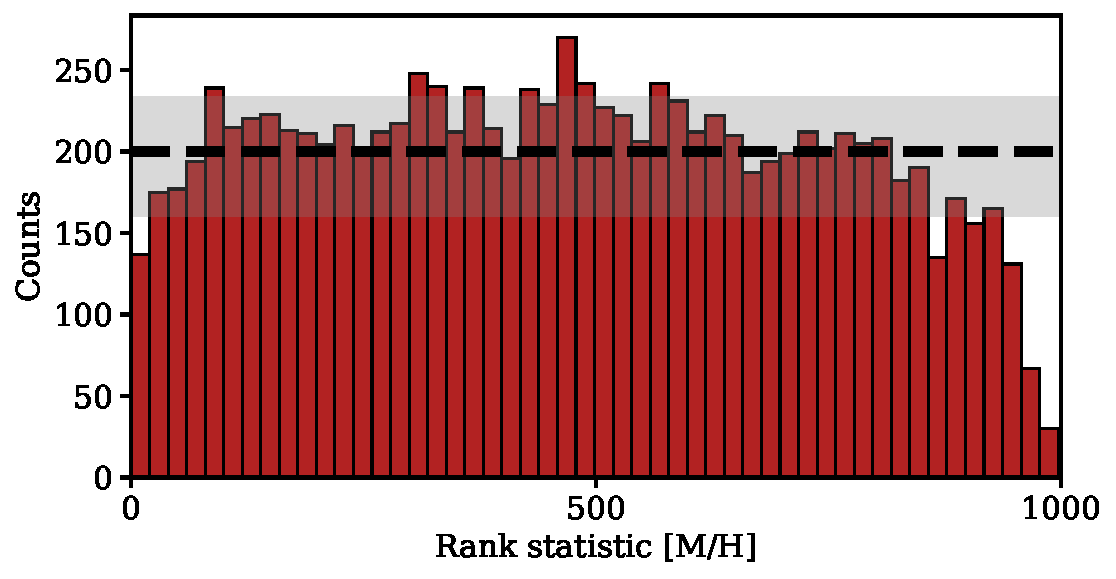
\includegraphics[width=0.45\textwidth]{images/sbc/rank_statisitic_4.pdf}
    
    
    
    \caption{Simulation-based calibration test of the posteriors for $1{,}000$ synthetic test observations. The red histograms in each panel represent the distribution of the rank statistic of the true value within the marginalised posterior for the percentiles $10\%$, $50\%$, $90\%$, and for $\rm{[M/H]}$. For a well calibrated posterior, the rank statistics will have a uniform distribution (black dashed line). A grey band indicates $99\%$ of the variation expected from a uniform histogram. The rank statistic distributions of our posteriors are nearly uniform for all of the four parameters, and therefore, the model provides unbiased and accurate posteriors.}

    \label{ranks}
\end{figure*}


\begin{figure}[h!]
    \centering
    
    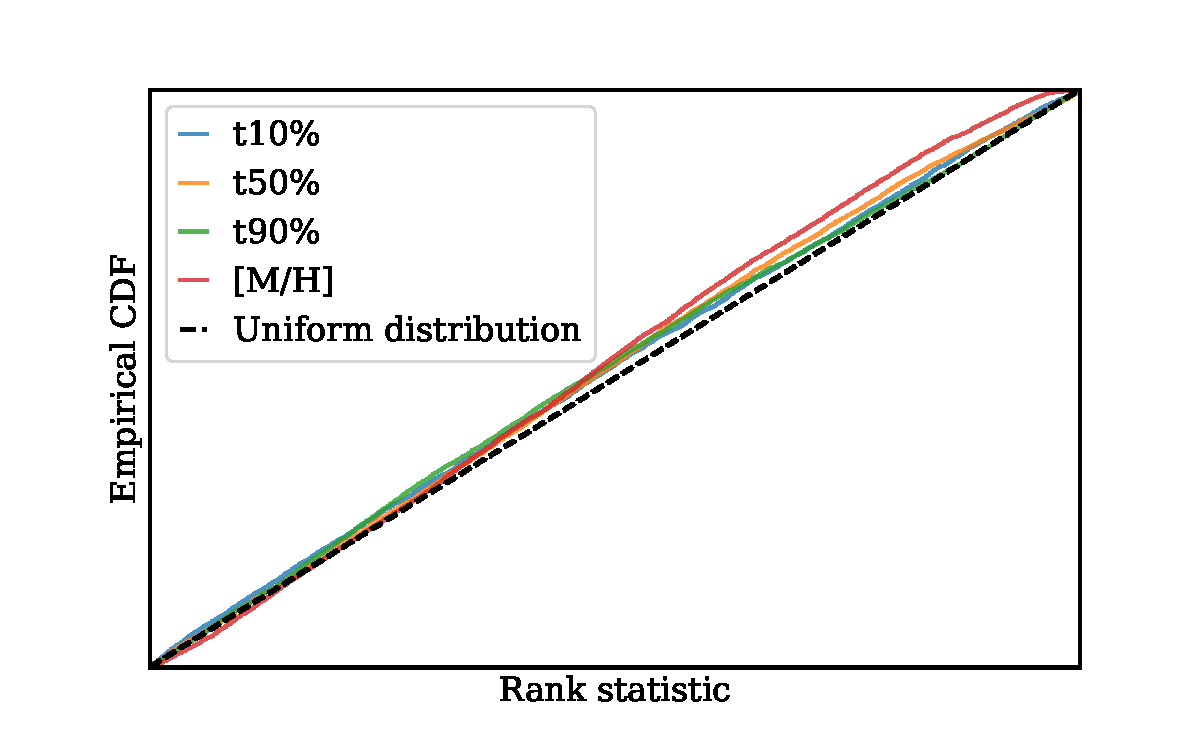
\includegraphics[width=0.5\textwidth]{images/sbc/ecdf.pdf}
    
    \caption{Empirical cumulative distribution functions (CDFs) for the percentiles $10\%$, $50\%$, $90\%$, and for $\rm{[M/H]}$, obtained with $1{,}000$ synthetic test observations.  If the posteriors are properly calibrated, the nominal coverage probability (percentage of probability volume), on the $x$-axis, would be equal to the coverage probability (percentage of actual values in such volume), on the $y$-axis, so the CDF is diagonal (black dashed line). Our CDFs are located very close to the diagonal, and the slight differences towards a conservative posterior, where the actual coverage probability is greater than the nominal coverage probability, allow the use of the model uncertainties as an upper limit. }

    \label{ecdf}
\end{figure}

\begin{figure}[h!]
    \centering
    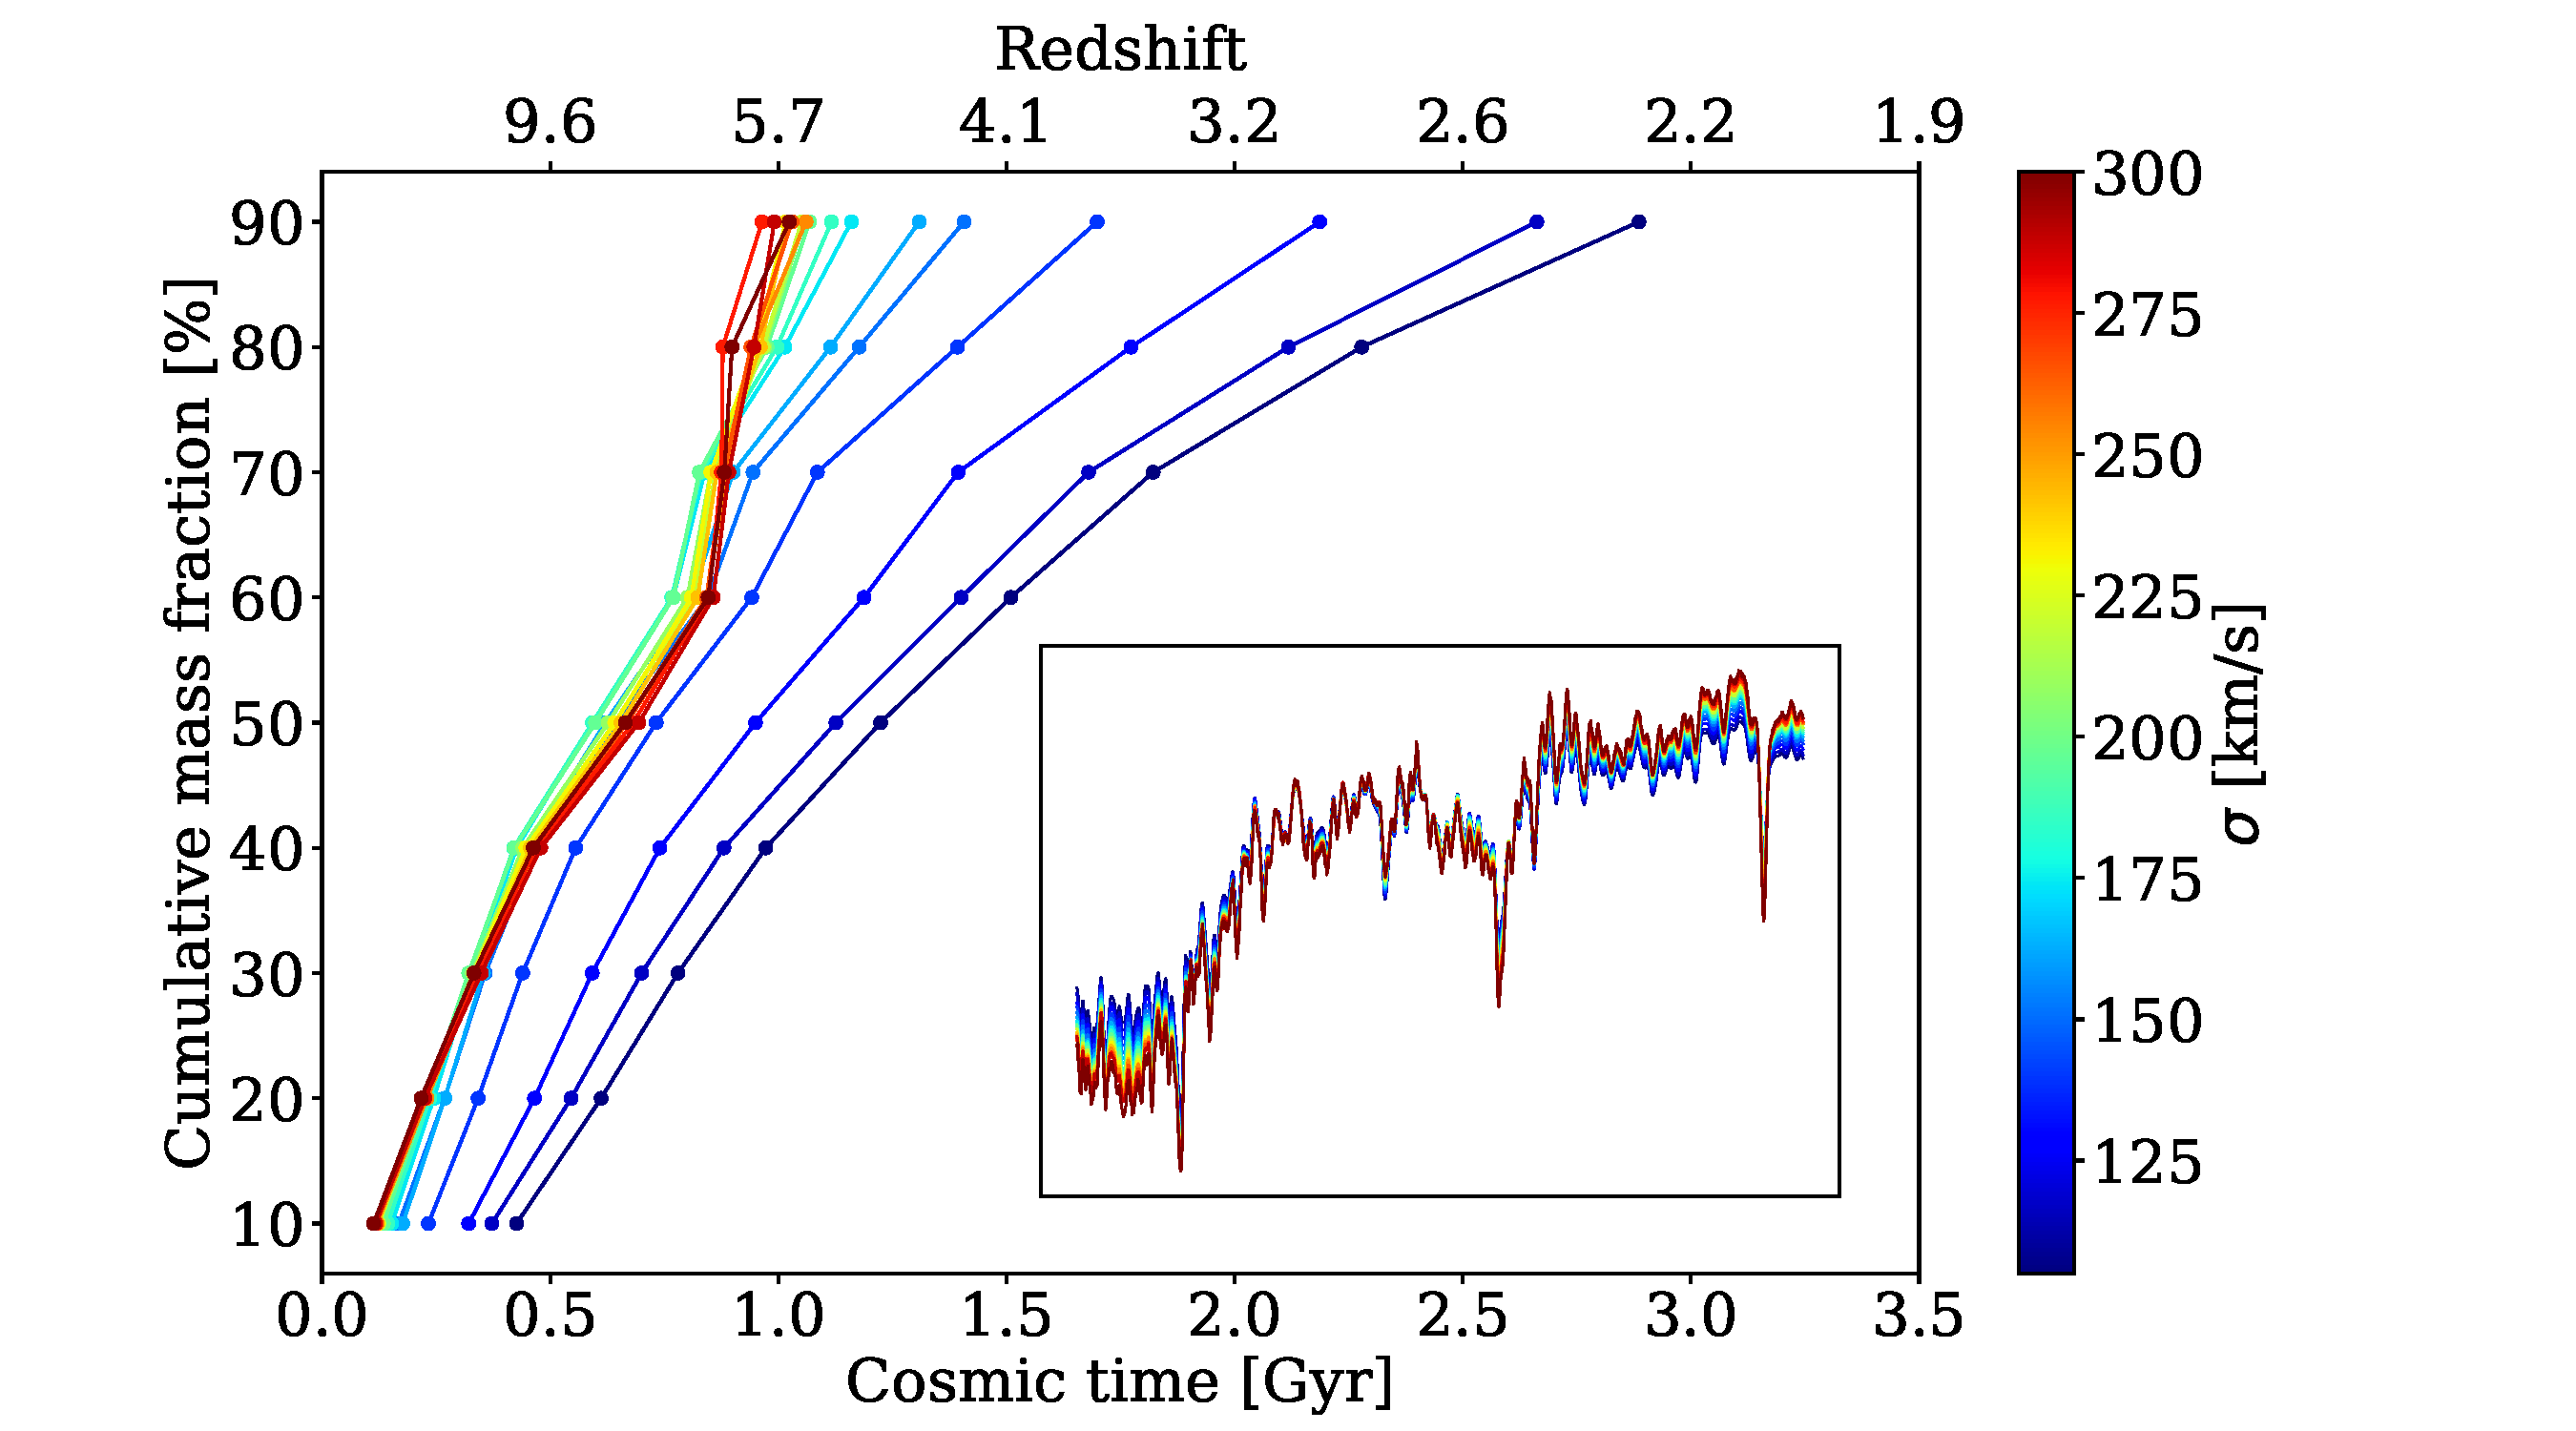
\includegraphics[width=0.5\textwidth]{images/obs/pred_gal_full.pdf}
    \caption{Median values of the posterior distributions obtained for the stellar mass percentiles of $18$ stacks, as a function of cosmic time in Gyr and redshift, coloured according to their velocity dispersions in km/s.  Redder colours are assigned to higher velocity dispersions (more massive galaxies), while bluer ones point to lower velocity dispersions (less massive ones). In the inset, we plot the observed spectra, normalised and in the wavelength range $[4023, 6000] \; \AA$, with the same colourmap.}
    \label{percentiles_obs_full}
\end{figure}



\begin{table}[h!]

\caption{Measurements of the model for 18 stacks with mean velocity dispersions in the range $105-300$ km/s. We include the cosmic time in Gyr at which $10$\%, $50$\%, and $90$\% of the total stellar mass are formed, as well as the metallicity $\rm{[M/H]}$. The values shown correspond to the median values of the predicted posterior distributions, and the uncertainties to the standard deviations.}
\centering
\resizebox{\hsize}{!}
            {
\begin{tblr}{
  cells = {c},
  hline{1,20} = {-}{0.08em},
  hline{2} = {-}{0.05em},
}

${\sigma}$ {[km/s]} & {P10\% [Gyr]} & {P50\% [Gyr]} & {P90\% [Gyr]} & $\rm{[M/H]}$ \\
100-110                            & 0.42$\pm0.22$         & 1.21$\pm0.34$        & 2.89$\pm0.63$        & 0.11$\pm0.24$   \\
110-120                            & 0.36$\pm0.22$        & 1.12$\pm0.32$        & 2.63$\pm0.66$        & 0.13$\pm0.23$  \\
120-130                            & 0.32$\pm0.21$        & 0.95$\pm0.33$        & 2.21$\pm0.75$        & -0.05$\pm0.32$ \\
130-140                            & 0.23$\pm0.17$        & 0.72$\pm0.29$        & 1.66$\pm0.70$         & -0.12$\pm0.40$  \\
140-150                            & 0.16$\pm0.13$        & 0.63$\pm0.24$        & 1.43$\pm0.57$        & 0.06$\pm0.38$  \\
150-160                            & 0.17$\pm0.13$        & 0.61$\pm0.25$        & 1.31$\pm0.61$        & -0.05$\pm0.39$ \\
160-170                            & 0.15$\pm0.12$        & 0.59$\pm0.21$        & 1.18$\pm0.54$        & 0.01$\pm0.40$   \\
170-180                            & 0.15$\pm0.11$        & 0.60$\pm0.21$         & 1.11$\pm0.53$        & -0.05$\pm0.40$  \\
180-190                            & 0.13$\pm0.10$         & 0.59$\pm0.20$         & 1.08$\pm0.50$         & -0.07$\pm0.41$ \\
190-200                            & 0.13$\pm0.09$        & 0.62$\pm0.18$        & 1.04$\pm0.46$        & 0.01$\pm0.37$  \\
200-210                            & 0.13$\pm0.11$         & 0.63$\pm0.16$       & 1.02$\pm0.41$        & -0.03$\pm0.39$  \\
210-220                            & 0.13$\pm0.10$         & 0.64$\pm0.17$        & 1.02$\pm0.44$        & -0.04$\pm0.37$ \\
220-230                            & 0.12$\pm0.09$        & 0.65$\pm0.15$        & 1.02$\pm0.42$        & -0.07$\pm0.37$ \\
230-240                            & 0.12$\pm0.12$        & 0.67$\pm0.14$        & 1.06$\pm0.39$        & 0.07$\pm0.37$  \\
240-250                            & 0.12$\pm0.07$        & 0.66$\pm0.12$        & 1.02$\pm0.39$        & 0.03$\pm0.38$  \\
250-260                            & 0.12$\pm0.07$        & 0.69$\pm0.11$        & 0.96$\pm0.36$        & 0.05$\pm0.39$  \\
260-280                            & 0.12$\pm0.06$        & 0.69$\pm0.12$        & 0.99$\pm0.41$        & -0.15$\pm0.38$ \\
280-320                            & 0.12$\pm0.07$         & 0.66$\pm0.11$        & 1.02$\pm0.37$       & 0.11$\pm0.34$

\end{tblr}}
\label{table_obs}
\end{table}


\begin{figure}[h!]
    \centering
    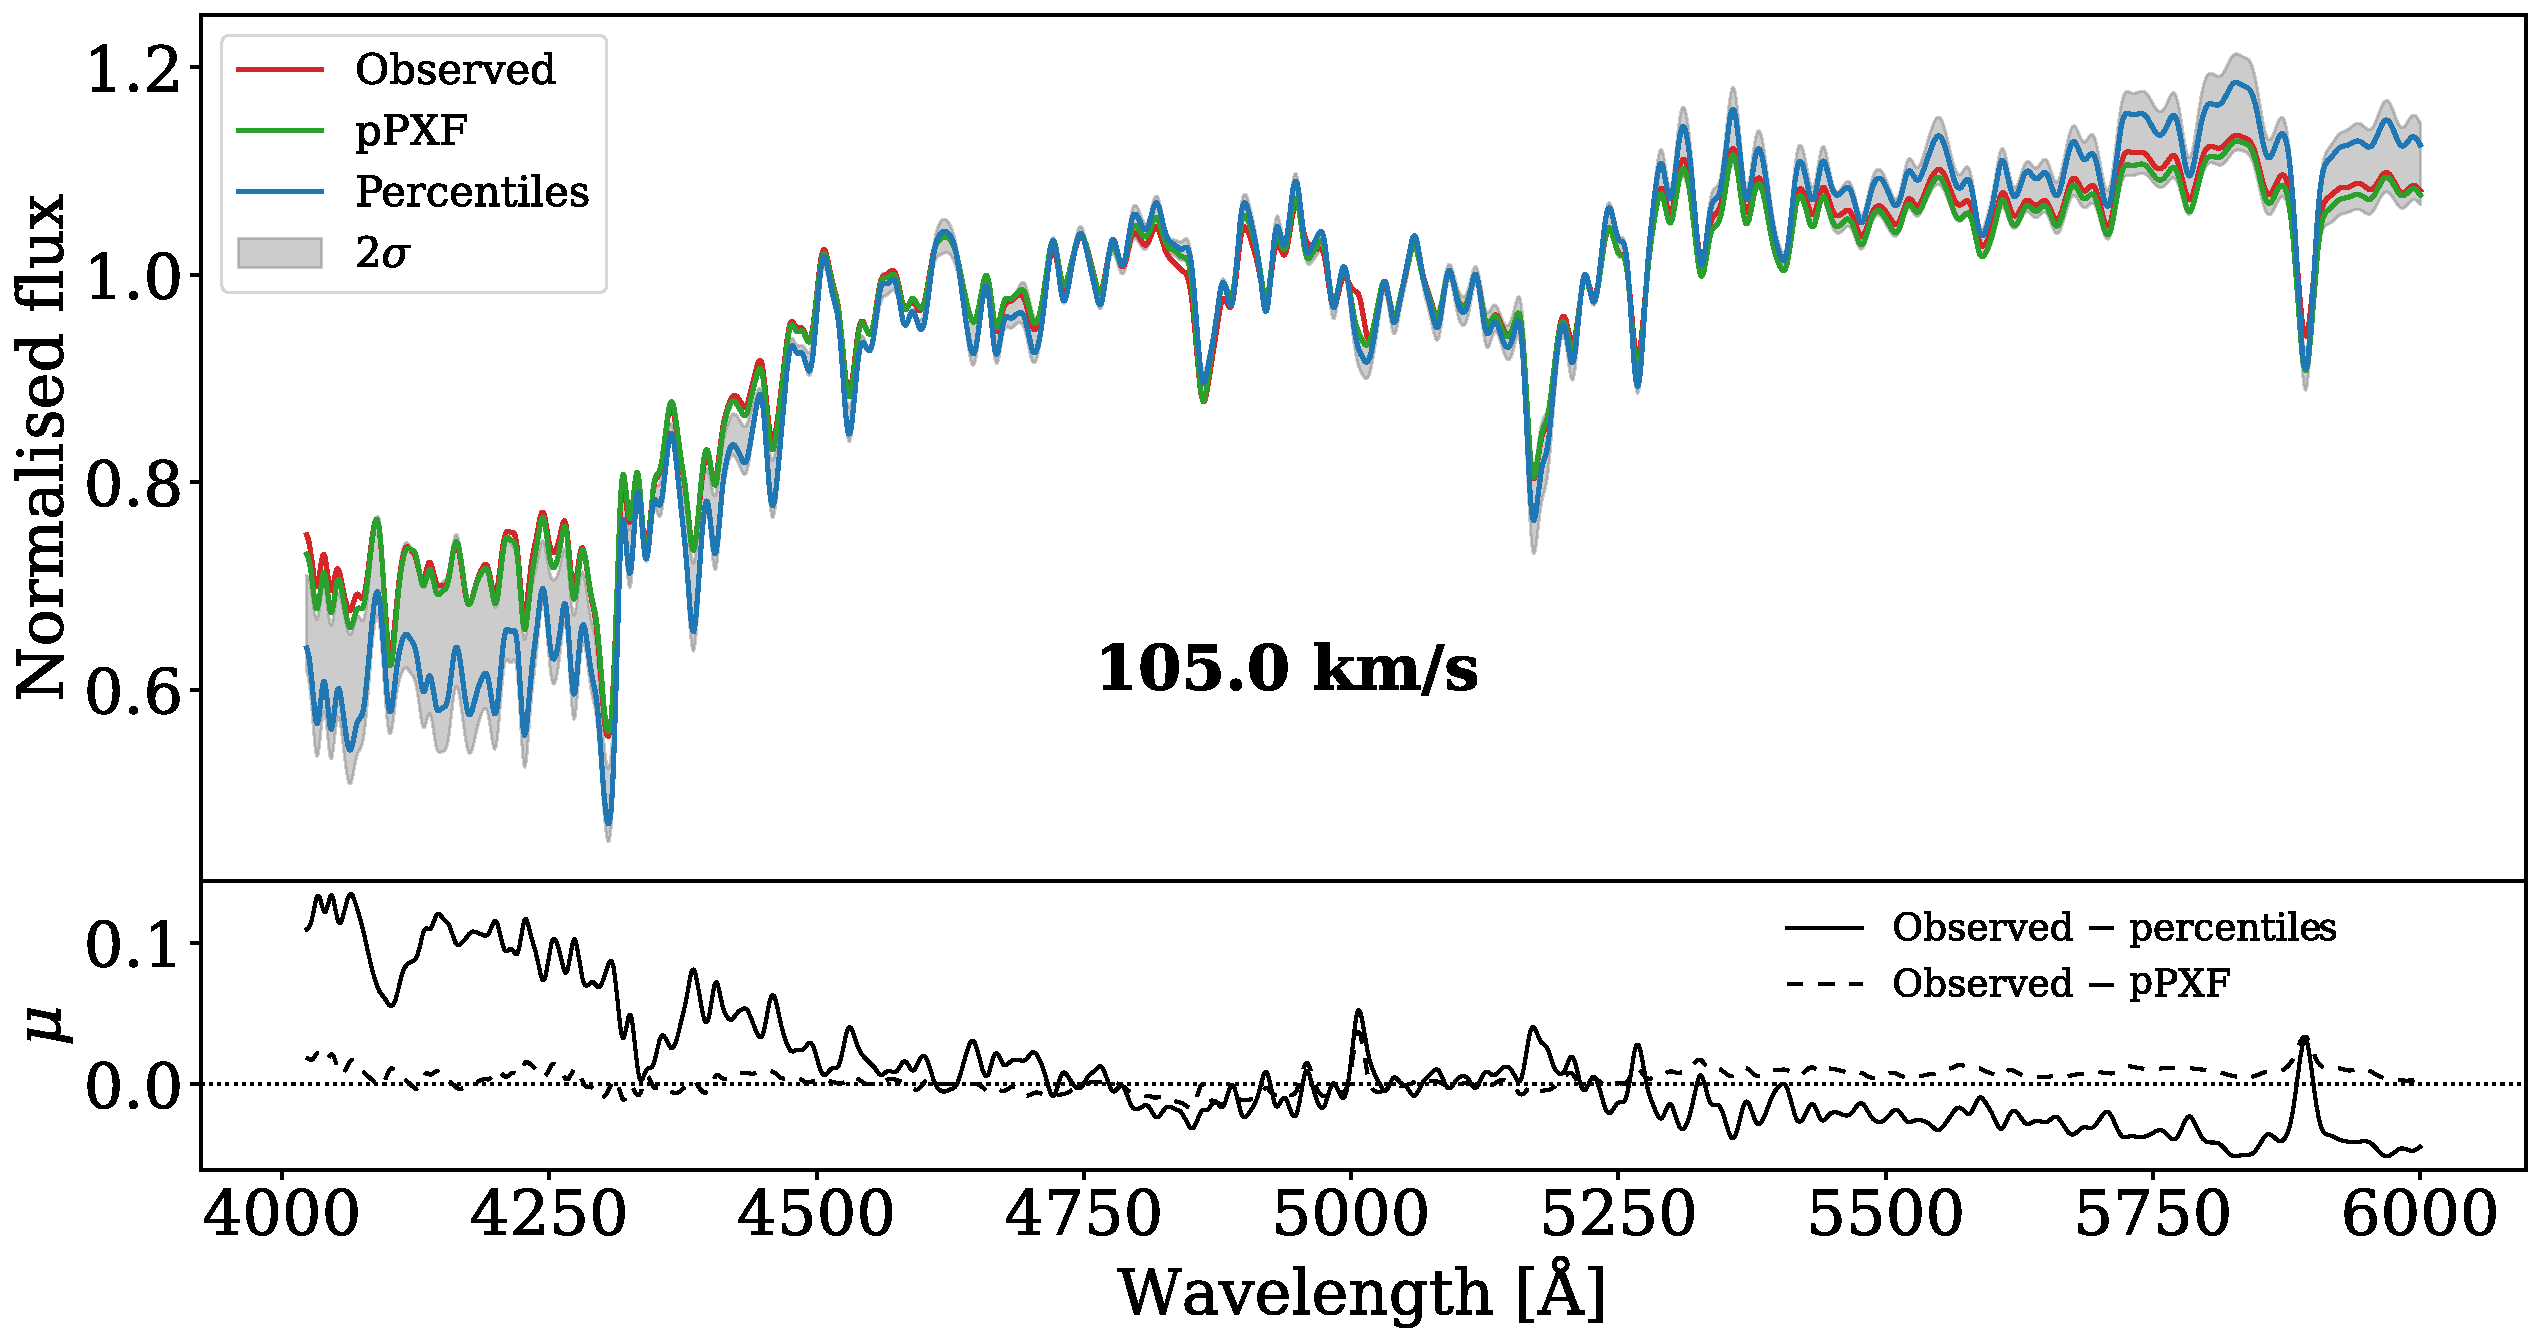
\includegraphics[width=0.5\textwidth]{images/obs/spectra_105.0_2.pdf}
    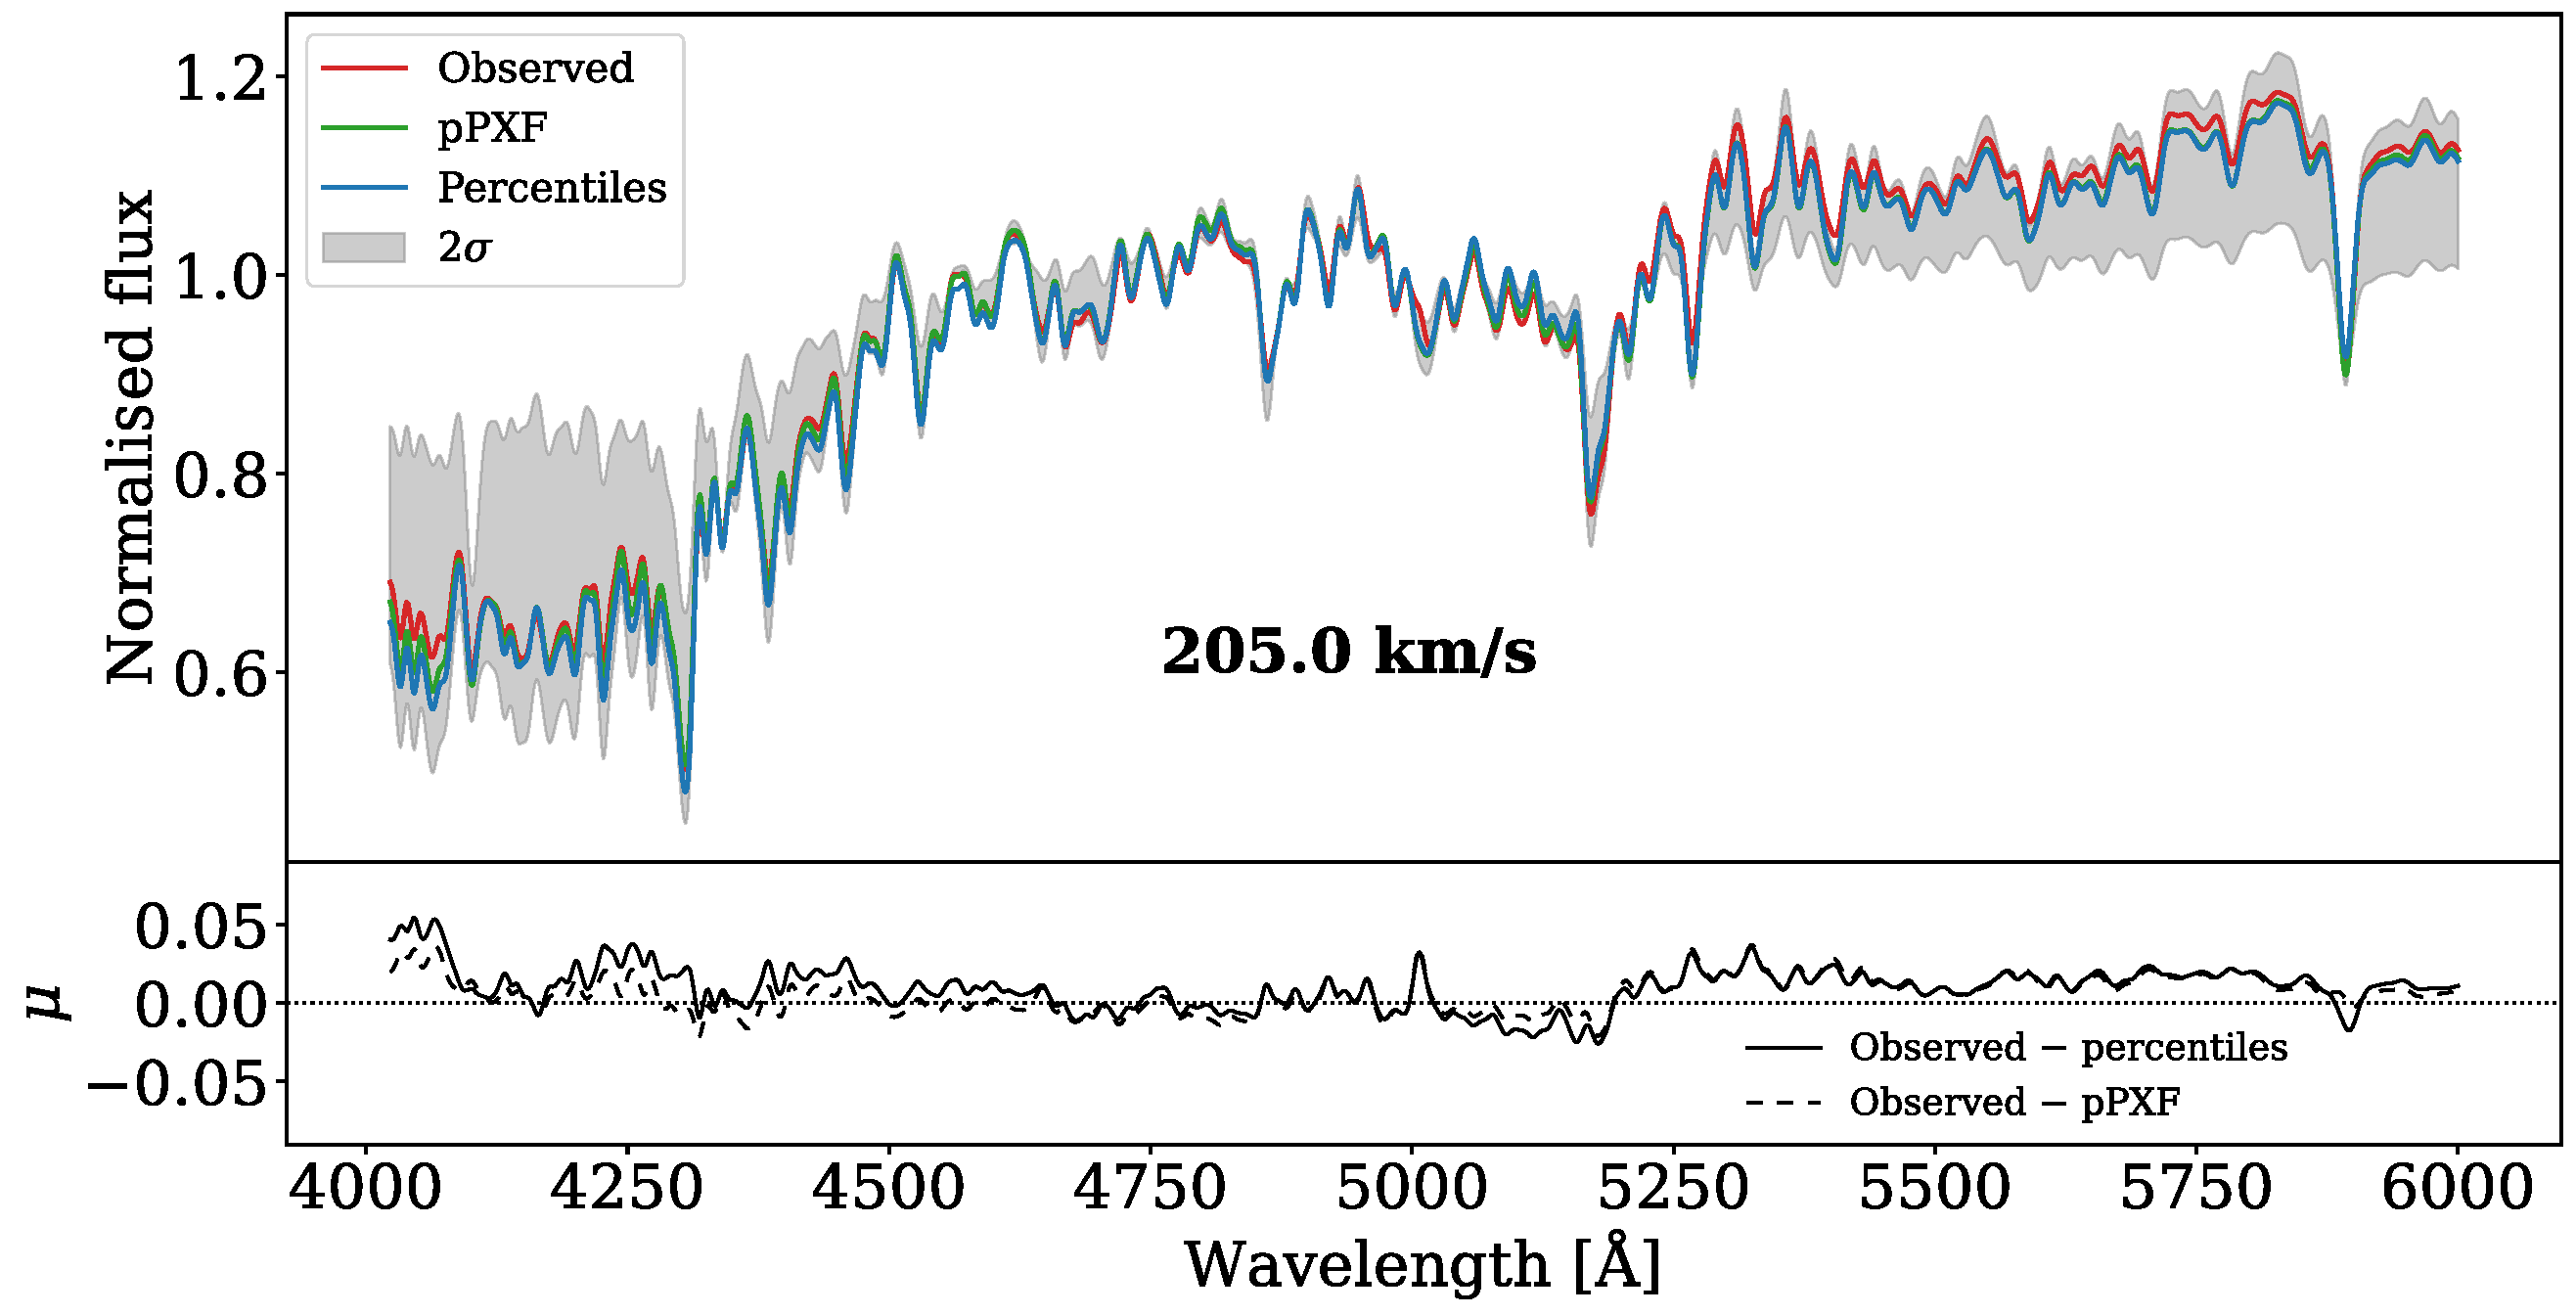
\includegraphics[width=0.5\textwidth]{images/obs/spectra_205.0_2.pdf}
    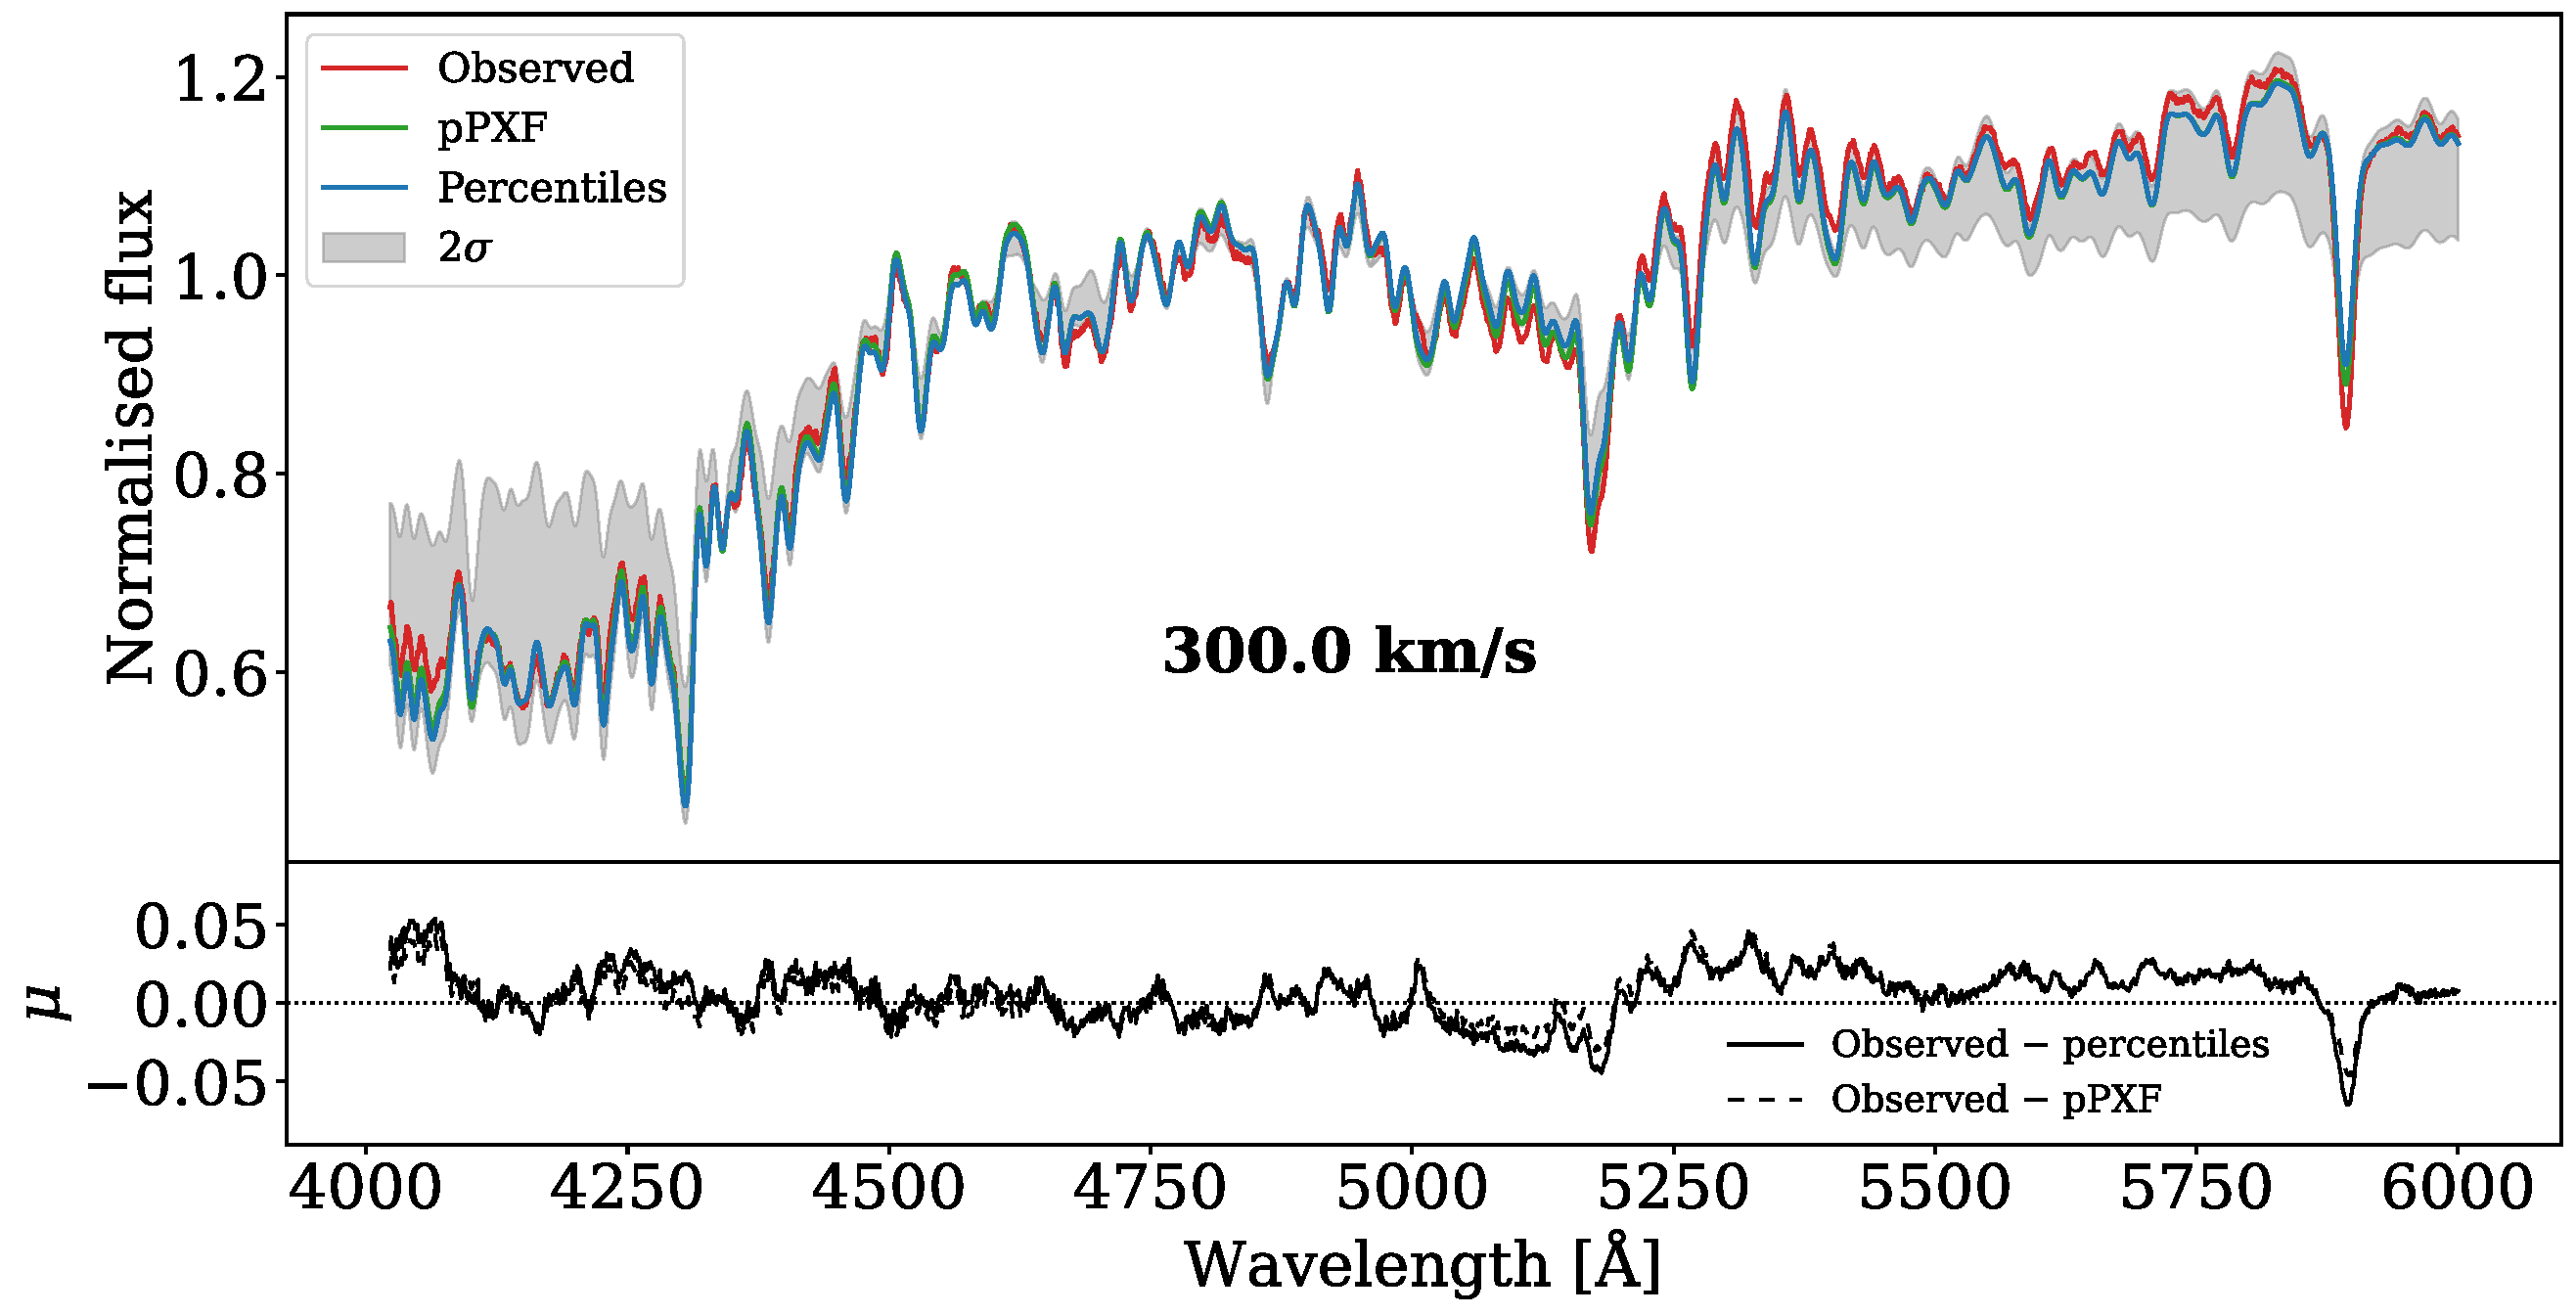
\includegraphics[width=0.5\textwidth]{images/obs/spectra_300.0_2.pdf}
    
    
    \caption{Reconstructions of the observed spectra for the stacks with velocity dispersion $105$, $205$ and $300$ km/s. In red we show the observed spectra, normalised by the median, in the wavelength range $[4023, 6000] \; \AA$. In blue, we show the spectra obtained as a linear combination of MILES SSP spectra according to our model, using the median values of the posteriors predicted. We repeat the procedure for the median $\pm2\sigma$ to get the grey-shadowed stripe, that shows how the uncertainties in the quantities measured are manifested in the spectra. In green, we plot the spectra obtained with the weights given by pPXF. In the lower panels, we include the residuals between the observed spectra and those reconstructed from the percentiles and metallicity predicted by our model (solid black line), and between the observed spectra and the one recovered by pPXF (dashed black line). The dotted line indicates the zero level. The typical value of the residuals of our method $(1.7\%)$ is very similar to the average value obtained with pPXF $(1.5\%)$, although in the first case the inference is performed in the latent space, without directly trying to reproduce the observed spectra.}
    \label{spectra_obs}
\end{figure}






%--------------------------------------------------------------------

\section{Discussion}

\label{discussion}

We have developed a new approach to estimate SFHs of galaxies from their optical absorption spectra, using simulation-based inference to obtain posteriors in a fully probabilistic treatment. From interpretable latent representations of the spectra, we predict the stellar mass  growth and metallicity, reaching high accuracy for the synthetic sample, as well as  properly calibrated uncertainties, evaluated through a SBC test. The predictions require less than half a second for each galaxy, sampling the posteriors with $1{,}000$ evaluations. This not only makes it possible to address a large dataset, but also to increase the number of evaluations for the posteriors, raising the precision of both the measurements and their uncertainties. \\


\subsection{Model considerations}

Although our new model is substantially faster than other Bayesian inference methods, such as MCMC, and provides well-calibrated uncertainties, unlike classical inversion methods applied to spectral fitting, it is subject to different systematics and modelling assumptions. One of the obvious limitations is the use of a forward model to train the network, because as our understanding of galaxy evolution is incomplete, the considerations taken when generating the synthetic data will never be fully constrained by a typical galaxy spectrum. Therefore, the prior, set by the distribution of parameters in the training set, will always have at least a moderate role in determining the answer. In particular, the simplifications made in terms of chemical evolution, by combining MILES SSP spectra with a fixed metallicity (instead of taking into account the metallicity histories) and working with base $\alpha$-enhancement models, may affect the reliability of our model predictions, given the intrinsic degeneration between the age and the metal content in the spectra. Moreover, there is currently no consensus on the stellar evolution \citep{Conroy_2009} or on the IMF of galaxies \citep{Mart_n_Navarro_2014}, and our model training has been restricted to a specific set of isochrones assuming a particular IMF parametrization. This limits the range of the training data, and dooms our model to fail in observations of galaxies that differ from these considerations.\\

It is known that the SFHs have a strong impact on the predicted posteriors, as shown by \cite{Leja_2019}, and models that mimic the breadth  distribution of SFR($t$) in the real Universe are required. In this work, in the pipeline provided by the GP-SFH module, we select a dispersive prior: a Dirichlet distribution with $\alpha=1.0$ for the fractional sSFR in each of the three equally-spaced time bins, positioning ourselves in favour of short-term variations in the SFHs (with smaller characteristic times). However, this selection must be explored with caution in future works.\\

On the other hand, a tuning of the backward model hyperparameters could be performed, among which we highlight the number of components of the latent representations in which we encode the spectrum, as well as the number of blocks used in the Masked Autoregressive Flow.


\subsection{Observations}

We obtain measurements of the SFH and the metallicity for stacks of SDSS spectra of ETGs. The model recovers the well-known relationship between  age and velocity dispersion, showing that the most massive galaxies ($\sigma \sim 300$ km/s) build up their stellar masses more abruptly, up to 90\% of their total stellar mass $1$ Gyr after the Big Bang, while the growth of stellar mass is softened in less massive galaxies. How these massive galaxies, up to $M_{*} \sim 10^{12} \, \rm M_{\odot}$ for the highest velocity dispersion stack, can form most of their masses so early is a question that is still open, given that a priori it requires a very high star formation efficiency. These galaxies are rare in the known Universe, with rapid bursts of star formation and followed by rapid quenching. The stars we see may have formed in different progenitor galaxies, which were located in the highest-density peaks of the Cosmic Web, and later assembled in major mergers \citep{conselice2007assembly}. To attend to these processes, hierarchical assembly models are necessary, commonly studied through large-scale cosmological simulations \citep[e.g.][]{Angeloudi_2023}. \\


As future work, we propose to measure SFHs and metallicities for late-type galaxies, for which we expect modelling difficulties due to the larger number of emission lines and potential `over-shining' effects when recovering the metallicity and ages of their first stars to form. So far we have not incorporated emission lines, noise models or dust attenuation, but including these aspects in the future is essential to manage a wide range of observations.  We can model the emission lines with specialised libraries \citep[e.g.][]{cloudy,fado}, or with data-driven approaches, training a neural network to  directly learn the relation between fundamental physical properties, such as stellar mass, SFR and metallicity, and observed emission features in real spectra. This last method can  also be extended to apply realistic noise to the spectra in the simulation, possibly introducing both the noisy spectra and the uncertainty distributions for the fluxes into the encoder, resulting in noise-aware latent representations.  In this way, we can condition the Bayesian inference with the noise.\\

Our approach can contribute, given its speed and error handling, to study the biases that produce features of the forward model that have traditionally been assumed in similar analyses. Following the first steps taken in this project for the stacks of SDSS spectra of ETGs, we plan to expand our model to  perform a deep sampling of current or upcoming spectroscopic surveys such as DESI \citep{desi}, WEAVE \citep{weave}, 4MOST \citep{4most}, or MOONS \citep{MOONS}, which will observe billions of galaxies and produce more than $10^8$ TB of data \citep{2023Smith}. 

%--------------------------------------------------------------------

\section{Summary and outlook}

By analysing the spectrum of a galaxy one can infer physical properties such as its stellar mass, star formation rates and chemical abundances, key ingredients of our understanding of galaxy evolution. State-of-the-art spectral fitting methods use MCMC sampling to perform Bayesian statistical inference, deriving posterior probability distributions of galaxy properties, given observations. However, obtaining a posterior sampled with $\sim 10{,}000$ evaluations with these methods requires $\gtrsim 1-10$ GPU hours per galaxy, and thus implies a major bottleneck for addressing large galaxy surveys. \\



We demonstrate in this work that an amortised simulation-based inference, with a previous encoding of the spectra, provides an alternative approach for spectral fitting through a neural density estimator. By using MILES templates and non-parametric SFHs, we construct a flexible model that recovers SFHs and metallicities with their uncertainties for observed stacks of spectra from  the SDSS, taking $\sim 4$\,s per galaxy to perform $10{,}000$ evaluations of the posteriors for the ten quantities we predict. The key results of our project are as follows.\\


    %Descripción del modelo
    
First, we construct a model composed of an encoder for the spectra based on a dot-product attention model, plus a Masked Autoregressive Flow, to estimate the posterior distributions for the cosmic time at which nine stellar mass percentiles are reached, and for the metallicity. We train it during $\sim4$ hours with $135{,}000$ synthetic samples obtained from SSP MILES templates and non-parametric SFHs from the GP-SFH module.\\

    % Descripción performance en datos sintéticos
    
 Second, we test the model with $15{,}000$ synthetic samples, reaching an $R^2$ score of $0.88$, $0.97$, $0.98$, and $0.96$ when estimating  the percentiles $10\%$, $50\%$, $90\%$, and the metallicity, respectively. The model recovers uncertainties associated with the degeneration of the inversion problem.  It struggles more in assessing the first percentiles in  galaxies with recent star formation, but reflects these difficulties adequately in the posteriors as indicated by an SBC test.\\
    

    %Observations
Third, we estimate with our model the SFHs and metallicities of $18$ stacks of ETGs from the SDSS, with a range of velocity dispersions of $105-300$ km/s,  as well as  reliable uncertainties for our measurements. We uncover very early bursts of star formation in the most massive galaxies, and a smoother growth of stellar mass when moving to intermediate masses, recovering the well-known relation between age and velocity dispersion. Moreover, we accurately reconstruct the spectra from MILES templates, using the nine ages and the mean metallicity measured, in good agreement with the real spectra with an averaged error of $1.7 \%$.\\

In future we plan to explore different sets of assumptions for the isochrones, the stellar library, and the IMF, as well as the effects of the priors introduced by the selection of SFHs and metallicity ranges. To simulate spectra of young stellar populations, a data-driven approach, possibly a neural network, can be used to directly learn the emission features from observed spectra. This methodology can also be extended to model the noise. To obtain noise-aware representations, the encoder may use both the uncertainties in the fluxes and the noisy spectra. At that stage, the optimal dimension of the latent vectors must be studied again. Such a complete model would allow one to analyse massive sets of galaxy spectra in a highly efficient and reliable manner.\\


The entire pipeline, including the scripts for the simulation and the Bayesian inference framework, is publicly available at \href{https://github.com/patriglesias/SBI_SFHs.git}{GitHub.}\footnote{\href{https://github.com/patriglesias/SBI_SFHs.git}{https://github.com/patriglesias/SBI\_SFHs.git}}


%--------------------------------------------------------------------

\begin{acknowledgements}

Co-funded by the European Union. Views and opinions expressed are however those of the author(s) only and do not necessarily reflect those of the European Union. Neither the European Union nor the granting authority can be held responsible for them. MHC and PIN acknowledge financial support from the State Research Agency (AEI\-MCINN) of the Spanish Ministry of Science and Innovation under the grants ``Galaxy Evolution with Artificial Intelligence" with reference PGC2018-100852-A-I00 and "BASALT" with reference PID2021-126838NB-I00. JHK acknowledges support from the Agencia Estatal de Investigaci\'on del Ministerio de Ciencia, Innovaci\'on y Universidades (MCIU/AEI) under the grant "The structure and evolution of galaxies and their outer regions" and the European Regional Development Fund (ERDF) with reference PID2022-136505NB-I00/10.13039/501100011033. EP acknowledges support from the Turning Scheme. 



\end{acknowledgements}


\bibliographystyle{aa}
\bibliography{references}
% WARNING
%-------------------------------------------------------------------
% Please note that we have included the references to the file aa.dem in
% order to compile it, but we ask you to:
%
% - use BibTeX with the regular commands:
%   \bibliographystyle{aa} % style aa.bst
%   \bibliography{Yourfile} % your references Yourfile.bib
%
% - join the .bib files when you upload your source files
%-------------------------------------------------------------------

%\input{appendix}

\end{document}
